\documentclass[acmsmall,review,nonacm]{acmart}
% Target: ACM Transactions on the Web (TWEB). `review` adds line numbers for submission.
\usepackage{booktabs,tabularx,multirow,longtable}
\usepackage{tikz}
\usetikzlibrary{positioning}
\setlength{\emergencystretch}{2em}
\newcommand{\todo}[1]{\textcolor{red}{[TODO: #1]}}
% Generated by make_numbers.py from testbed/results/revision; do not edit.
\newcommand{\AfiveShift}{0.005}
\newcommand{\AfiveShiftMax}{0.005}
\newcommand{\AfiveViews}{52{,}224}
\newcommand{\AfourFourSeed}{8}
\newcommand{\AfourNavPninetyNine}{1.0--1.9}
\newcommand{\AfourRidgeSig}{1}
\newcommand{\AfourSig}{12}
\newcommand{\AfourSigFour}{5}
\newcommand{\AfourStaleCells}{34}
\newcommand{\AfourStaleIn}{31}
\newcommand{\AfourTests}{16}
\newcommand{\AfourTie}{3}
\newcommand{\AfourTieFour}{3}
\newcommand{\AfourTwoSeed}{8}
\newcommand{\AoneAbunReal}{4.3--4.8}
\newcommand{\AoneFullHome}{5.3--8.3}
\newcommand{\AoneFullHone}{0.33--1.23}
\newcommand{\AoneNoRhoHome}{3.8--6.4}
\newcommand{\AoneNoRhoHone}{0.98--2.81}
\newcommand{\AoneNoRhoQ}{2.2--2.6}
\newcommand{\AoneNoRhoRtwo}{4.7--7.9}
\newcommand{\AoneNoRhoVnine}{19.3}
\newcommand{\AoneNoRhoVnineb}{4.6--6.3}
\newcommand{\AonePooledQ}{4.5--7.0}
\newcommand{\AoneServiceAll}{49--96}
\newcommand{\AtwoModelWins}{13}
\newcommand{\AtwoOutCells}{0}
\newcommand{\AtwoRidge}{0.17--3.61}
\newcommand{\AtwoTests}{16}
\newcommand{\AtwoTrees}{1.4--26.4}
\newcommand{\BfourCalibRuns}{32}
\newcommand{\BfourOffMaxRegret}{0.0}
\newcommand{\BfourOffNocache}{17--42}
\newcommand{\BoneOffBrier}{0.073--0.093}
\newcommand{\BoneOffSkill}{0.57--0.76}
\newcommand{\BoneOffTop}{93--95}
\newcommand{\ccCells}{140}
\newcommand{\ccRBrier}{0.074}
\newcommand{\ccRCcConf}{0}
\newcommand{\ccRCcDec}{6}
\newcommand{\ccRCcRegret}{7.1}
\newcommand{\ccRCcRight}{1}
\newcommand{\ccRCcViol}{0}
\newcommand{\ccRCcWorst}{14.9}
\newcommand{\ccRExcess}{0.014}
\newcommand{\ccRFails}{W2, B4cc-a}
\newcommand{\ccRLone}{1.12}
\newcommand{\ccRLtwo}{3.76}
\newcommand{\ccRMarginConf}{0}
\newcommand{\ccRMarginDec}{6}
\newcommand{\ccRMarginMax}{0.046}
\newcommand{\ccRMarginMin}{0.015}
\newcommand{\ccRMarginRegret}{7.1}
\newcommand{\ccRMarginRight}{1}
\newcommand{\ccRMarginViol}{0}
\newcommand{\ccRMarginWorst}{14.9}
\newcommand{\ccROonePrime}{passed}
\newcommand{\ccRPointConf}{0}
\newcommand{\ccRPointDec}{6}
\newcommand{\ccRPointRegret}{4.6}
\newcommand{\ccRPointRight}{2}
\newcommand{\ccRPointViol}{0}
\newcommand{\ccRPointWorst}{6.9}
\newcommand{\ccRSame}{6}
\newcommand{\ccRSkill}{0.69}
\newcommand{\ccRTop}{94.6}
\newcommand{\ccRVerdict}{failed}
\newcommand{\ccRWone}{0.019}
\newcommand{\ccRWthree}{97 of 97}
\newcommand{\ccRWtwo}{0.066}
\newcommand{\ccRmsSds}{0.022}
\newcommand{\ccRmse}{0.024}
\newcommand{\ccSdm}{0.0084}
\newcommand{\ccTBrier}{0.087}
\newcommand{\ccTCcConf}{0}
\newcommand{\ccTCcDec}{10}
\newcommand{\ccTCcRegret}{4.0}
\newcommand{\ccTCcRight}{3}
\newcommand{\ccTCcViol}{0}
\newcommand{\ccTCcWorst}{11.6}
\newcommand{\ccTExcess}{0.026}
\newcommand{\ccTFails}{W2}
\newcommand{\ccTLone}{1.01}
\newcommand{\ccTLtwo}{3.06}
\newcommand{\ccTMarginConf}{0}
\newcommand{\ccTMarginDec}{10}
\newcommand{\ccTMarginMax}{0.044}
\newcommand{\ccTMarginMin}{0.015}
\newcommand{\ccTMarginRegret}{4.0}
\newcommand{\ccTMarginRight}{3}
\newcommand{\ccTMarginViol}{0}
\newcommand{\ccTMarginWorst}{11.6}
\newcommand{\ccTOonePrime}{passed}
\newcommand{\ccTPointConf}{0}
\newcommand{\ccTPointDec}{10}
\newcommand{\ccTPointRegret}{1.1}
\newcommand{\ccTPointRight}{5}
\newcommand{\ccTPointViol}{3}
\newcommand{\ccTPointWorst}{6.4}
\newcommand{\ccTSame}{10}
\newcommand{\ccTSkill}{0.67}
\newcommand{\ccTTop}{94.1}
\newcommand{\ccTVerdict}{failed}
\newcommand{\ccTWone}{0.013}
\newcommand{\ccTWthree}{99 of 99}
\newcommand{\ccTWtwo}{0.052}
\newcommand{\ccWithin}{90}
\newcommand{\cdHRBrier}{0.034}
\newcommand{\cdHRDecisions}{4}
\newcommand{\cdHRDefaultRegret}{0.2}
\newcommand{\cdHRDefaultViol}{3}
\newcommand{\cdHRExcess}{0.010}
\newcommand{\cdHRFails}{W3}
\newcommand{\cdHRFixedRegret}{0.5}
\newcommand{\cdHRFixedViol}{0}
\newcommand{\cdHRLone}{1.34}
\newcommand{\cdHRLtwo}{5.78}
\newcommand{\cdHRNocacheRegret}{2.9}
\newcommand{\cdHRNocacheViol}{0}
\newcommand{\cdHRRegret}{0.55}
\newcommand{\cdHRRegretWorst}{1.43}
\newcommand{\cdHRSkill}{0.91}
\newcommand{\cdHRTop}{98.0}
\newcommand{\cdHRTuningRegret}{--}
\newcommand{\cdHRTuningViol}{0}
\newcommand{\cdHRVerdict}{failed}
\newcommand{\cdHRViol}{0}
\newcommand{\cdHRWone}{0.012}
\newcommand{\cdHRWthree}{258 of 260}
\newcommand{\cdHRWtwo}{0.043}
\newcommand{\cdHRZeroBrier}{0.072}
\newcommand{\cdHRZeroDecisions}{4}
\newcommand{\cdHRZeroDefaultRegret}{0.2}
\newcommand{\cdHRZeroDefaultViol}{3}
\newcommand{\cdHRZeroExcess}{0.051}
\newcommand{\cdHRZeroFails}{L1, L2, O1, O3}
\newcommand{\cdHRZeroFixedRegret}{0.5}
\newcommand{\cdHRZeroFixedViol}{0}
\newcommand{\cdHRZeroLone}{16.47}
\newcommand{\cdHRZeroLtwo}{23.33}
\newcommand{\cdHRZeroNocacheRegret}{2.9}
\newcommand{\cdHRZeroNocacheViol}{0}
\newcommand{\cdHRZeroRegret}{0.55}
\newcommand{\cdHRZeroRegretWorst}{1.43}
\newcommand{\cdHRZeroSkill}{0.81}
\newcommand{\cdHRZeroTop}{96.1}
\newcommand{\cdHRZeroTuningRegret}{--}
\newcommand{\cdHRZeroTuningViol}{0}
\newcommand{\cdHRZeroVerdict}{failed}
\newcommand{\cdHRZeroViol}{0}
\newcommand{\cdHRZeroWone}{0.014}
\newcommand{\cdHRZeroWthree}{248 of 248}
\newcommand{\cdHRZeroWtwo}{0.043}
\newcommand{\cdHTBrier}{0.048}
\newcommand{\cdHTDecisions}{4}
\newcommand{\cdHTDefaultRegret}{--}
\newcommand{\cdHTDefaultViol}{4}
\newcommand{\cdHTExcess}{0.008}
\newcommand{\cdHTFails}{O1}
\newcommand{\cdHTFixedRegret}{0.5}
\newcommand{\cdHTFixedViol}{0}
\newcommand{\cdHTLone}{0.80}
\newcommand{\cdHTLtwo}{2.68}
\newcommand{\cdHTNocacheRegret}{1.3}
\newcommand{\cdHTNocacheViol}{0}
\newcommand{\cdHTRegret}{0.05}
\newcommand{\cdHTRegretWorst}{0.20}
\newcommand{\cdHTSkill}{0.88}
\newcommand{\cdHTTop}{96.6}
\newcommand{\cdHTTuningRegret}{--}
\newcommand{\cdHTTuningViol}{0}
\newcommand{\cdHTVerdict}{failed}
\newcommand{\cdHTViol}{0}
\newcommand{\cdHTWone}{0.011}
\newcommand{\cdHTWthree}{287 of 287}
\newcommand{\cdHTWtwo}{0.040}
\newcommand{\cdHTZeroBrier}{0.081}
\newcommand{\cdHTZeroDecisions}{4}
\newcommand{\cdHTZeroDefaultRegret}{--}
\newcommand{\cdHTZeroDefaultViol}{4}
\newcommand{\cdHTZeroExcess}{0.042}
\newcommand{\cdHTZeroFails}{L1, L2, O3}
\newcommand{\cdHTZeroFixedRegret}{0.5}
\newcommand{\cdHTZeroFixedViol}{0}
\newcommand{\cdHTZeroLone}{8.06}
\newcommand{\cdHTZeroLtwo}{13.20}
\newcommand{\cdHTZeroNocacheRegret}{1.3}
\newcommand{\cdHTZeroNocacheViol}{0}
\newcommand{\cdHTZeroRegret}{0.05}
\newcommand{\cdHTZeroRegretWorst}{0.20}
\newcommand{\cdHTZeroSkill}{0.80}
\newcommand{\cdHTZeroTop}{95.0}
\newcommand{\cdHTZeroTuningRegret}{--}
\newcommand{\cdHTZeroTuningViol}{0}
\newcommand{\cdHTZeroVerdict}{failed}
\newcommand{\cdHTZeroViol}{0}
\newcommand{\cdHTZeroWone}{0.012}
\newcommand{\cdHTZeroWthree}{287 of 287}
\newcommand{\cdHTZeroWtwo}{0.037}
\newcommand{\cdRBrier}{0.034}
\newcommand{\cdRDecisions}{4}
\newcommand{\cdRDefaultRegret}{0.4}
\newcommand{\cdRDefaultViol}{3}
\newcommand{\cdRExcess}{0.004}
\newcommand{\cdRFails}{W2, W3, O1}
\newcommand{\cdRFixedRegret}{0.2}
\newcommand{\cdRFixedViol}{0}
\newcommand{\cdRLone}{1.39}
\newcommand{\cdRLtwo}{3.04}
\newcommand{\cdRNocacheRegret}{0.7}
\newcommand{\cdRNocacheViol}{0}
\newcommand{\cdRRegret}{0.17}
\newcommand{\cdRRegretWorst}{0.26}
\newcommand{\cdRSkill}{0.91}
\newcommand{\cdRTop}{97.8}
\newcommand{\cdRTuningRegret}{0.1}
\newcommand{\cdRTuningViol}{0}
\newcommand{\cdRVerdict}{failed}
\newcommand{\cdRViol}{0}
\newcommand{\cdRWone}{0.013}
\newcommand{\cdRWthree}{266 of 267}
\newcommand{\cdRWtwo}{0.060}
\newcommand{\cdRZeroBrier}{0.037}
\newcommand{\cdRZeroDecisions}{4}
\newcommand{\cdRZeroDefaultRegret}{0.4}
\newcommand{\cdRZeroDefaultViol}{3}
\newcommand{\cdRZeroExcess}{0.007}
\newcommand{\cdRZeroFails}{W2, W3}
\newcommand{\cdRZeroFixedRegret}{0.2}
\newcommand{\cdRZeroFixedViol}{0}
\newcommand{\cdRZeroLone}{1.87}
\newcommand{\cdRZeroLtwo}{5.30}
\newcommand{\cdRZeroNocacheRegret}{0.7}
\newcommand{\cdRZeroNocacheViol}{0}
\newcommand{\cdRZeroRegret}{0.17}
\newcommand{\cdRZeroRegretWorst}{0.26}
\newcommand{\cdRZeroSkill}{0.91}
\newcommand{\cdRZeroTop}{97.6}
\newcommand{\cdRZeroTuningRegret}{--}
\newcommand{\cdRZeroTuningViol}{0}
\newcommand{\cdRZeroVerdict}{failed}
\newcommand{\cdRZeroViol}{0}
\newcommand{\cdRZeroWone}{0.013}
\newcommand{\cdRZeroWthree}{266 of 267}
\newcommand{\cdRZeroWtwo}{0.063}
\newcommand{\cdTBrier}{0.049}
\newcommand{\cdTDecisions}{4}
\newcommand{\cdTDefaultRegret}{0.1}
\newcommand{\cdTDefaultViol}{3}
\newcommand{\cdTExcess}{0.007}
\newcommand{\cdTFails}{O1}
\newcommand{\cdTFixedRegret}{0.1}
\newcommand{\cdTFixedViol}{0}
\newcommand{\cdTLone}{1.39}
\newcommand{\cdTLtwo}{3.90}
\newcommand{\cdTNocacheRegret}{0.4}
\newcommand{\cdTNocacheViol}{0}
\newcommand{\cdTRegret}{0.00}
\newcommand{\cdTRegretWorst}{0.00}
\newcommand{\cdTSkill}{0.88}
\newcommand{\cdTTop}{96.5}
\newcommand{\cdTTuningRegret}{0.0}
\newcommand{\cdTTuningViol}{0}
\newcommand{\cdTVerdict}{failed}
\newcommand{\cdTViol}{0}
\newcommand{\cdTWone}{0.011}
\newcommand{\cdTWthree}{281 of 281}
\newcommand{\cdTWtwo}{0.036}
\newcommand{\cdTZeroBrier}{0.049}
\newcommand{\cdTZeroDecisions}{4}
\newcommand{\cdTZeroDefaultRegret}{0.1}
\newcommand{\cdTZeroDefaultViol}{3}
\newcommand{\cdTZeroExcess}{0.008}
\newcommand{\cdTZeroFails}{O1}
\newcommand{\cdTZeroFixedRegret}{0.1}
\newcommand{\cdTZeroFixedViol}{0}
\newcommand{\cdTZeroLone}{0.76}
\newcommand{\cdTZeroLtwo}{3.12}
\newcommand{\cdTZeroNocacheRegret}{0.4}
\newcommand{\cdTZeroNocacheViol}{0}
\newcommand{\cdTZeroRegret}{0.19}
\newcommand{\cdTZeroRegretWorst}{0.26}
\newcommand{\cdTZeroSkill}{0.88}
\newcommand{\cdTZeroTop}{96.5}
\newcommand{\cdTZeroTuningRegret}{--}
\newcommand{\cdTZeroTuningViol}{0}
\newcommand{\cdTZeroVerdict}{failed}
\newcommand{\cdTZeroViol}{0}
\newcommand{\cdTZeroWone}{0.011}
\newcommand{\cdTZeroWthree}{281 of 281}
\newcommand{\cdTZeroWtwo}{0.038}
\newcommand{\decBlindSig}{4}
\newcommand{\decBlocks}{10}
\newcommand{\decCalfreqSig}{1}
\newcommand{\decCatBlindConf}{0}
\newcommand{\decCatBlindExc}{0.00}
\newcommand{\decCatBlindMean}{5.0}
\newcommand{\decCatBlindN}{32}
\newcommand{\decCatBlindViol}{0}
\newcommand{\decCatBlindWorst}{23.4}
\newcommand{\decCatCalfreqConf}{0}
\newcommand{\decCatCalfreqExc}{0.00}
\newcommand{\decCatCalfreqMean}{1.1}
\newcommand{\decCatCalfreqN}{32}
\newcommand{\decCatCalfreqViol}{0}
\newcommand{\decCatCalfreqWorst}{13.7}
\newcommand{\decCatDefaultExc}{0.85}
\newcommand{\decCatDefaultMean}{0.2}
\newcommand{\decCatDefaultN}{32}
\newcommand{\decCatDefaultViol}{29}
\newcommand{\decCatDefaultWorst}{0.4}
\newcommand{\decCatFixedExc}{0.00}
\newcommand{\decCatFixedMean}{1.8}
\newcommand{\decCatFixedN}{32}
\newcommand{\decCatFixedViol}{0}
\newcommand{\decCatFixedWorst}{13.7}
\newcommand{\decCatModelConf}{0}
\newcommand{\decCatModelExc}{0.00}
\newcommand{\decCatModelMean}{0.4}
\newcommand{\decCatModelN}{32}
\newcommand{\decCatModelViol}{0}
\newcommand{\decCatModelWorst}{2.0}
\newcommand{\decCatNocacheExc}{0.00}
\newcommand{\decCatNocacheMean}{10.4}
\newcommand{\decCatNocacheN}{32}
\newcommand{\decCatNocacheViol}{0}
\newcommand{\decCatNocacheWorst}{32.1}
\newcommand{\decCatRidgeConf}{0}
\newcommand{\decCatRidgeExc}{0.00}
\newcommand{\decCatRidgeMean}{0.4}
\newcommand{\decCatRidgeN}{32}
\newcommand{\decCatRidgeViol}{0}
\newcommand{\decCatRidgeWorst}{2.0}
\newcommand{\decCatScen}{8}
\newcommand{\decCatSimpleConf}{10}
\newcommand{\decCatSimpleExc}{0.19}
\newcommand{\decCatSimpleMean}{0.8}
\newcommand{\decCatSimpleN}{32}
\newcommand{\decCatSimpleViol}{10}
\newcommand{\decCatSimpleWorst}{3.9}
\newcommand{\decCatSingleConf}{12}
\newcommand{\decCatSingleExc}{0.19}
\newcommand{\decCatSingleMean}{0.4}
\newcommand{\decCatSingleN}{32}
\newcommand{\decCatSingleViol}{12}
\newcommand{\decCatSingleWorst}{2.0}
\newcommand{\decCatTuningExc}{0.00}
\newcommand{\decCatTuningMean}{0.4}
\newcommand{\decCatTuningN}{24}
\newcommand{\decCatTuningViol}{0}
\newcommand{\decCatTuningWorst}{4.2}
\newcommand{\decCcBlindConf}{0}
\newcommand{\decCcBlindExc}{0.00}
\newcommand{\decCcBlindMean}{6.5}
\newcommand{\decCcBlindN}{16}
\newcommand{\decCcBlindViol}{0}
\newcommand{\decCcBlindWorst}{14.9}
\newcommand{\decCcCalfreqConf}{0}
\newcommand{\decCcCalfreqExc}{0.00}
\newcommand{\decCcCalfreqMean}{5.7}
\newcommand{\decCcCalfreqN}{16}
\newcommand{\decCcCalfreqViol}{0}
\newcommand{\decCcCalfreqWorst}{14.9}
\newcommand{\decCcModelConf}{0}
\newcommand{\decCcModelExc}{0.00}
\newcommand{\decCcModelMean}{5.1}
\newcommand{\decCcModelN}{16}
\newcommand{\decCcModelViol}{0}
\newcommand{\decCcModelWorst}{14.9}
\newcommand{\decCcPtBlindConf}{0}
\newcommand{\decCcPtBlindExc}{0.00}
\newcommand{\decCcPtBlindMean}{4.5}
\newcommand{\decCcPtBlindN}{16}
\newcommand{\decCcPtBlindViol}{1}
\newcommand{\decCcPtBlindWorst}{10.4}
\newcommand{\decCcPtCalfreqConf}{0}
\newcommand{\decCcPtCalfreqExc}{0.00}
\newcommand{\decCcPtCalfreqMean}{2.4}
\newcommand{\decCcPtCalfreqN}{16}
\newcommand{\decCcPtCalfreqViol}{1}
\newcommand{\decCcPtCalfreqWorst}{7.0}
\newcommand{\decCcPtModelConf}{0}
\newcommand{\decCcPtModelExc}{0.02}
\newcommand{\decCcPtModelMean}{2.7}
\newcommand{\decCcPtModelN}{16}
\newcommand{\decCcPtModelViol}{3}
\newcommand{\decCcPtModelWorst}{6.9}
\newcommand{\decCcPtRidgeConf}{0}
\newcommand{\decCcPtRidgeExc}{0.02}
\newcommand{\decCcPtRidgeMean}{2.7}
\newcommand{\decCcPtRidgeN}{16}
\newcommand{\decCcPtRidgeViol}{3}
\newcommand{\decCcPtRidgeWorst}{6.9}
\newcommand{\decCcPtScen}{4}
\newcommand{\decCcPtSimpleConf}{4}
\newcommand{\decCcPtSimpleExc}{0.08}
\newcommand{\decCcPtSimpleMean}{1.2}
\newcommand{\decCcPtSimpleN}{16}
\newcommand{\decCcPtSimpleViol}{6}
\newcommand{\decCcPtSimpleWorst}{11.6}
\newcommand{\decCcPtSingleConf}{4}
\newcommand{\decCcPtSingleExc}{0.08}
\newcommand{\decCcPtSingleMean}{1.2}
\newcommand{\decCcPtSingleN}{16}
\newcommand{\decCcPtSingleViol}{6}
\newcommand{\decCcPtSingleWorst}{11.6}
\newcommand{\decCcRidgeConf}{0}
\newcommand{\decCcRidgeExc}{0.00}
\newcommand{\decCcRidgeMean}{5.1}
\newcommand{\decCcRidgeN}{16}
\newcommand{\decCcRidgeViol}{0}
\newcommand{\decCcRidgeWorst}{14.9}
\newcommand{\decCcScen}{4}
\newcommand{\decCcSimpleConf}{4}
\newcommand{\decCcSimpleExc}{0.08}
\newcommand{\decCcSimpleMean}{2.7}
\newcommand{\decCcSimpleN}{16}
\newcommand{\decCcSimpleViol}{6}
\newcommand{\decCcSimpleWorst}{14.9}
\newcommand{\decCcSingleConf}{4}
\newcommand{\decCcSingleExc}{0.08}
\newcommand{\decCcSingleMean}{2.7}
\newcommand{\decCcSingleN}{16}
\newcommand{\decCcSingleViol}{6}
\newcommand{\decCcSingleWorst}{14.9}
\newcommand{\decHardBlindConf}{0}
\newcommand{\decHardBlindExc}{0.00}
\newcommand{\decHardBlindMean}{12.0}
\newcommand{\decHardBlindN}{16}
\newcommand{\decHardBlindViol}{0}
\newcommand{\decHardBlindWorst}{25.7}
\newcommand{\decHardCalfreqConf}{0}
\newcommand{\decHardCalfreqExc}{0.00}
\newcommand{\decHardCalfreqMean}{6.1}
\newcommand{\decHardCalfreqN}{16}
\newcommand{\decHardCalfreqViol}{0}
\newcommand{\decHardCalfreqWorst}{15.6}
\newcommand{\decHardModelConf}{0}
\newcommand{\decHardModelExc}{0.00}
\newcommand{\decHardModelMean}{4.9}
\newcommand{\decHardModelN}{16}
\newcommand{\decHardModelViol}{0}
\newcommand{\decHardModelWorst}{11.0}
\newcommand{\decHardPtBlindConf}{0}
\newcommand{\decHardPtBlindExc}{0.00}
\newcommand{\decHardPtBlindMean}{11.5}
\newcommand{\decHardPtBlindN}{16}
\newcommand{\decHardPtBlindViol}{0}
\newcommand{\decHardPtBlindWorst}{25.7}
\newcommand{\decHardPtCalfreqConf}{0}
\newcommand{\decHardPtCalfreqExc}{0.02}
\newcommand{\decHardPtCalfreqMean}{4.6}
\newcommand{\decHardPtCalfreqN}{16}
\newcommand{\decHardPtCalfreqViol}{1}
\newcommand{\decHardPtCalfreqWorst}{15.6}
\newcommand{\decHardPtModelConf}{0}
\newcommand{\decHardPtModelExc}{0.02}
\newcommand{\decHardPtModelMean}{2.9}
\newcommand{\decHardPtModelN}{16}
\newcommand{\decHardPtModelViol}{3}
\newcommand{\decHardPtModelWorst}{10.5}
\newcommand{\decHardPtRidgeConf}{0}
\newcommand{\decHardPtRidgeExc}{0.02}
\newcommand{\decHardPtRidgeMean}{2.9}
\newcommand{\decHardPtRidgeN}{16}
\newcommand{\decHardPtRidgeViol}{3}
\newcommand{\decHardPtRidgeWorst}{10.5}
\newcommand{\decHardPtScen}{4}
\newcommand{\decHardPtSimpleConf}{5}
\newcommand{\decHardPtSimpleExc}{0.14}
\newcommand{\decHardPtSimpleMean}{2.5}
\newcommand{\decHardPtSimpleN}{16}
\newcommand{\decHardPtSimpleViol}{8}
\newcommand{\decHardPtSimpleWorst}{11.0}
\newcommand{\decHardPtSingleConf}{5}
\newcommand{\decHardPtSingleExc}{0.14}
\newcommand{\decHardPtSingleMean}{2.5}
\newcommand{\decHardPtSingleN}{16}
\newcommand{\decHardPtSingleViol}{8}
\newcommand{\decHardPtSingleWorst}{11.0}
\newcommand{\decHardRidgeConf}{0}
\newcommand{\decHardRidgeExc}{0.00}
\newcommand{\decHardRidgeMean}{4.9}
\newcommand{\decHardRidgeN}{16}
\newcommand{\decHardRidgeViol}{0}
\newcommand{\decHardRidgeWorst}{11.0}
\newcommand{\decHardScen}{4}
\newcommand{\decHardSimpleConf}{3}
\newcommand{\decHardSimpleExc}{0.08}
\newcommand{\decHardSimpleMean}{2.0}
\newcommand{\decHardSimpleN}{16}
\newcommand{\decHardSimpleViol}{6}
\newcommand{\decHardSimpleWorst}{11.0}
\newcommand{\decHardSingleConf}{3}
\newcommand{\decHardSingleExc}{0.08}
\newcommand{\decHardSingleMean}{2.0}
\newcommand{\decHardSingleN}{16}
\newcommand{\decHardSingleViol}{6}
\newcommand{\decHardSingleWorst}{11.0}
\newcommand{\decLoneGap}{0.07}
\newcommand{\decLonePred}{0.80--1.75}
\newcommand{\decLoneTrue}{0.77--1.74}
\newcommand{\decRidgeSig}{0}
\newcommand{\decSingleSig}{6}
\newcommand{\diagDecTraceRate}{0.063}
\newcommand{\diagDecTraceTotal}{0.122}
\newcommand{\diagDecrevBTwoTDeclared}{0.026}
\newcommand{\diagDecrevBTwoTRealized}{0.033}
\newcommand{\diagDecrevRDeclared}{0.020}
\newcommand{\diagDecrevRRealized}{0.019}
\newcommand{\diagDecrevTDeclared}{0.016}
\newcommand{\diagDecrevTRealized}{0.015}
\newcommand{\diagNoiseRDeciles}{5}
\newcommand{\diagNoiseRExcl}{2}
\newcommand{\diagNoiseRHalf}{0.012--0.046}
\newcommand{\diagNoiseRMaxExcl}{0.061}
\newcommand{\diagNoiseTDeciles}{9}
\newcommand{\diagNoiseTExcl}{3}
\newcommand{\diagNoiseTHalf}{0.022--0.054}
\newcommand{\diagNoiseTMaxExcl}{0.066}
\newcommand{\diagPushRFormula}{0.162}
\newcommand{\diagPushRNoWriteCache}{99.3}
\newcommand{\diagPushRObs}{0.152}
\newcommand{\diagPushRPredR}{0.180}
\newcommand{\diagPushRPredRtwo}{0.172}
\newcommand{\diagPushRWriteFetched}{100}
\newcommand{\diagPushTFormula}{0.370}
\newcommand{\diagPushTNoWriteCache}{97.7}
\newcommand{\diagPushTObs}{0.369}
\newcommand{\diagPushTPredR}{0.406}
\newcommand{\diagPushTPredRtwo}{0.388}
\newcommand{\diagPushTWriteFetched}{100}
\newcommand{\diagTraceDeclared}{2.5}
\newcommand{\diagTraceRate}{1.8--2.1}
\newcommand{\distcdRLoneDec}{1.18}
\newcommand{\distcdRLoneDist}{1.35}
\newcommand{\distcdRWoneDec}{0.012}
\newcommand{\distcdRWoneDist}{0.013}
\newcommand{\distcdTLoneDec}{1.01}
\newcommand{\distcdTLoneDist}{1.08}
\newcommand{\distcdTWoneDec}{0.011}
\newcommand{\distcdTWoneDist}{0.010}
\newcommand{\distrevRLoneDec}{1.64}
\newcommand{\distrevRLoneDist}{1.77}
\newcommand{\distrevRWoneDec}{0.020}
\newcommand{\distrevRWoneDist}{0.020}
\newcommand{\distrevTLoneDec}{1.28}
\newcommand{\distrevTLoneDist}{1.23}
\newcommand{\distrevTWoneDec}{0.016}
\newcommand{\distrevTWoneDist}{0.016}
\newcommand{\marginFiveAbst}{0}
\newcommand{\marginFiveDec}{16}
\newcommand{\marginFiveRegret}{4.9}
\newcommand{\marginFiveRight}{6}
\newcommand{\marginFiveViol}{0}
\newcommand{\marginSevenAbst}{1}
\newcommand{\marginSevenDec}{16}
\newcommand{\marginSevenRegret}{5.6}
\newcommand{\marginSevenRight}{4}
\newcommand{\marginSevenViol}{0}
\newcommand{\marginThreeAbst}{0}
\newcommand{\marginThreeDec}{16}
\newcommand{\marginThreeRegret}{4.9}
\newcommand{\marginThreeRight}{6}
\newcommand{\marginThreeViol}{0}
\newcommand{\marginTwoAbst}{0}
\newcommand{\marginTwoDec}{16}
\newcommand{\marginTwoRegret}{4.9}
\newcommand{\marginTwoRight}{6}
\newcommand{\marginTwoViol}{0}
\newcommand{\marginUpper}{17}
\newcommand{\marginZeroAbst}{0}
\newcommand{\marginZeroDec}{16}
\newcommand{\marginZeroRegret}{2.9}
\newcommand{\marginZeroRight}{8}
\newcommand{\marginZeroViol}{3}
\newcommand{\revBTwoRBrier}{0.108}
\newcommand{\revBTwoRExcess}{-0.000}
\newcommand{\revBTwoRFails}{W2, W3, O1}
\newcommand{\revBTwoRInside}{10 of 12}
\newcommand{\revBTwoRLone}{1.48}
\newcommand{\revBTwoRLtwo}{4.06}
\newcommand{\revBTwoROnoffMae}{0.030}
\newcommand{\revBTwoROnoffMax}{0.051}
\newcommand{\revBTwoRPeriodicMae}{0.003}
\newcommand{\revBTwoRPeriodicMax}{0.004}
\newcommand{\revBTwoRSkill}{0.56}
\newcommand{\revBTwoRTop}{93.3}
\newcommand{\revBTwoRTraceMae}{0.021}
\newcommand{\revBTwoRTraceMax}{0.047}
\newcommand{\revBTwoRVerdict}{failed}
\newcommand{\revBTwoRWone}{0.018}
\newcommand{\revBTwoRWthree}{46 of 47}
\newcommand{\revBTwoRWtwo}{0.051}
\newcommand{\revBTwoTBrier}{0.167}
\newcommand{\revBTwoTExcess}{0.019}
\newcommand{\revBTwoTFails}{W2, W3, O1}
\newcommand{\revBTwoTInside}{7 of 12}
\newcommand{\revBTwoTLone}{1.30}
\newcommand{\revBTwoTLtwo}{2.86}
\newcommand{\revBTwoTOnoffMae}{0.007}
\newcommand{\revBTwoTOnoffMax}{0.016}
\newcommand{\revBTwoTPeriodicMae}{0.020}
\newcommand{\revBTwoTPeriodicMax}{0.038}
\newcommand{\revBTwoTSkill}{0.55}
\newcommand{\revBTwoTTop}{87.4}
\newcommand{\revBTwoTTraceMae}{0.050}
\newcommand{\revBTwoTTraceMax}{0.122}
\newcommand{\revBTwoTVerdict}{failed}
\newcommand{\revBTwoTWone}{0.026}
\newcommand{\revBTwoTWthree}{52 of 53}
\newcommand{\revBTwoTWtwo}{0.122}
\newcommand{\revHRAwareConf}{0}
\newcommand{\revHRAwareDec}{8}
\newcommand{\revHRAwareRegret}{5.8}
\newcommand{\revHRAwareRight}{3}
\newcommand{\revHRAwareViol}{0}
\newcommand{\revHRAwareWorst}{10.5}
\newcommand{\revHRBrier}{0.075}
\newcommand{\revHRExcess}{0.015}
\newcommand{\revHRFails}{B4h-a}
\newcommand{\revHRLone}{0.96}
\newcommand{\revHRLtwo}{2.88}
\newcommand{\revHRNaiveConf}{0}
\newcommand{\revHRNaiveDec}{8}
\newcommand{\revHRNaiveRegret}{4.9}
\newcommand{\revHRNaiveRight}{3}
\newcommand{\revHRNaiveViol}{2}
\newcommand{\revHRNaiveWorst}{10.5}
\newcommand{\revHROonePrime}{passed}
\newcommand{\revHRSkill}{0.75}
\newcommand{\revHRTop}{94.6}
\newcommand{\revHRVerdict}{failed}
\newcommand{\revHRWone}{0.013}
\newcommand{\revHRWthree}{91 of 91}
\newcommand{\revHRWtwo}{0.031}
\newcommand{\revHTAwareConf}{0}
\newcommand{\revHTAwareDec}{8}
\newcommand{\revHTAwareRegret}{4.1}
\newcommand{\revHTAwareRight}{3}
\newcommand{\revHTAwareViol}{0}
\newcommand{\revHTAwareWorst}{11.0}
\newcommand{\revHTBrier}{0.086}
\newcommand{\revHTExcess}{0.025}
\newcommand{\revHTFails}{none}
\newcommand{\revHTLone}{1.75}
\newcommand{\revHTLtwo}{5.59}
\newcommand{\revHTNaiveConf}{0}
\newcommand{\revHTNaiveDec}{8}
\newcommand{\revHTNaiveRegret}{1.2}
\newcommand{\revHTNaiveRight}{5}
\newcommand{\revHTNaiveViol}{1}
\newcommand{\revHTNaiveWorst}{8.5}
\newcommand{\revHTOonePrime}{passed}
\newcommand{\revHTSkill}{0.68}
\newcommand{\revHTTop}{93.9}
\newcommand{\revHTVerdict}{passed}
\newcommand{\revHTWone}{0.011}
\newcommand{\revHTWthree}{99 of 99}
\newcommand{\revHTWtwo}{0.029}
\newcommand{\revRBrier}{0.046}
\newcommand{\revRDecisions}{8}
\newcommand{\revRDefaultRegret}{--}
\newcommand{\revRDefaultViol}{8}
\newcommand{\revRExcess}{0.010}
\newcommand{\revRFails}{W2, W3, O1}
\newcommand{\revRFixedRegret}{2.0}
\newcommand{\revRFixedViol}{0}
\newcommand{\revRInside}{45 of 54}
\newcommand{\revRLone}{1.50}
\newcommand{\revRLtwo}{4.36}
\newcommand{\revRNocacheRegret}{17.9}
\newcommand{\revRNocacheViol}{0}
\newcommand{\revRRegret}{0.46}
\newcommand{\revRRegretWorst}{1.09}
\newcommand{\revRSkill}{0.77}
\newcommand{\revRTop}{97.0}
\newcommand{\revRTuningRegret}{0.5}
\newcommand{\revRTuningViol}{0}
\newcommand{\revRVerdict}{failed}
\newcommand{\revRViol}{0}
\newcommand{\revRWone}{0.020}
\newcommand{\revRWthree}{1132 of 1134}
\newcommand{\revRWtwo}{0.082}
\newcommand{\revTBrier}{0.065}
\newcommand{\revTDecisions}{8}
\newcommand{\revTDefaultRegret}{--}
\newcommand{\revTDefaultViol}{8}
\newcommand{\revTExcess}{0.021}
\newcommand{\revTFails}{W2, O1}
\newcommand{\revTFixedRegret}{4.4}
\newcommand{\revTFixedViol}{0}
\newcommand{\revTInside}{44 of 54}
\newcommand{\revTLone}{1.47}
\newcommand{\revTLtwo}{7.04}
\newcommand{\revTNocacheRegret}{21.3}
\newcommand{\revTNocacheViol}{0}
\newcommand{\revTRegret}{0.60}
\newcommand{\revTRegretWorst}{2.00}
\newcommand{\revTSkill}{0.77}
\newcommand{\revTTop}{95.5}
\newcommand{\revTTuningRegret}{0.6}
\newcommand{\revTTuningViol}{0}
\newcommand{\revTVerdict}{failed}
\newcommand{\revTViol}{0}
\newcommand{\revTWone}{0.016}
\newcommand{\revTWthree}{1191 of 1191}
\newcommand{\revTWtwo}{0.052}


\acmJournal{TWEB}
\setcopyright{none}
\settopmatter{printacmref=false, printfolios=true}

\title{Predicting Latency and Freshness of Cached Client- and Server-Rendered Web Applications}
\subtitle{Which Cache Layer Answers, What It Costs, and Which Policy to Choose}

\author{Istiak Ahmed Tashrif}
\orcid{0009-0001-6363-4129}
\email{istiaktashrif@gmail.com}
\affiliation{%
  \department{Department of Computer Science and Engineering}
  \institution{Sonargaon University}
  \streetaddress{147/I, Green Road, Panthapath, Tejgaon}
  \city{Dhaka}
  \postcode{1205}
  \country{Bangladesh}}

\begin{abstract}
Whether a web page shows its data sooner with client-side rendering (CSR) or server-side rendering (SSR), and how often that data is out of date, depends on which of several stacked caches answers each request, on the network, and on how much work the server does. We present a predictor that, before a workload runs, derives for every user action which cache layer serves it (browser, framework, application cache or database), the time until its data is visible, and the probability that it shows stale data, from the cache policies, a description of the workload (its session distribution and write process, as could be estimated from past traffic) and round-trip times measured on the path. Every prediction is written before its run, on conditions never used for fitting, and every version is tested again on an independent replication; all versions, including failures, are reported. Latency is predicted within 0.2--1.8\% mean error across emulated paths, one real relayed internet path in three configurations (HTTP/1.1, measured bandwidth, and HTTPS with HTTP/2), a second framework, a heavier page, and an independently written second application (RealWorld Conduit) on two hosts, including when the serving layer must be predicted under TTL expiry and push invalidation. Equal-information baselines show that most of this accuracy comes from knowing which layer serves each action; mechanistic path terms add a smaller margin that matters on real paths. Pooled stale-view shares are predicted within 0.006--0.026 absolute error. Stricter per-cell and calibration criteria were first missed; a post-hoc diagnosis traced part of the miss to how the model timed cache exposure, and the corrected model, frozen and tested on fresh blocks with predictions from the session distribution alone, passed every prediction criterion on its two fresh tests. Predictions still fail when a trace's write rate drifts from its history. Used to choose among 27 rendering and caching policies under a staleness limit, the predictions selected policies within 2\% of the observed best in every test with the 27-candidate set, with no limit violations, whereas framework-default TTLs violated the limit in 29 of 32 decisions; with limits placed at the predicted boundary, a selector with a staleness margin stayed within every limit at 4--6\% latency regret. We also report where prediction fails (consumer broadband, shared-core concurrency, throttled devices) and measurement pitfalls that distort such studies.
\end{abstract}

\begin{CCSXML}
<ccs2012>
   <concept>
       <concept_id>10002951.10003260.10003282</concept_id>
       <concept_desc>Information systems~Web applications</concept_desc>
       <concept_significance>500</concept_significance>
       </concept>
   <concept>
       <concept_id>10003033.10003079.10003080</concept_id>
       <concept_desc>Networks~Network performance modeling</concept_desc>
       <concept_significance>500</concept_significance>
       </concept>
   <concept>
       <concept_id>10003033.10003079.10011704</concept_id>
       <concept_desc>Networks~Network measurement</concept_desc>
       <concept_significance>300</concept_significance>
       </concept>
   <concept>
       <concept_id>10003033.10003079.10011672</concept_id>
       <concept_desc>Networks~Network performance analysis</concept_desc>
       <concept_significance>300</concept_significance>
       </concept>
 </ccs2012>
\end{CCSXML}

\ccsdesc[500]{Information systems~Web applications}
\ccsdesc[500]{Networks~Network performance modeling}
\ccsdesc[300]{Networks~Network measurement}
\ccsdesc[300]{Networks~Network performance analysis}

\keywords{web performance, server-side rendering, client-side rendering, caching, cache invalidation, staleness, performance modeling, prospective validation}

\begin{document}
\maketitle

% =====================================================================
\section{Introduction}

Modern web frameworks let developers choose, per page, whether data is fetched and rendered in the browser (client-side rendering, CSR) or on the server (server-side rendering, SSR), and they offer several caches on each path: a per-user browser cache (e.g.\ TanStack Query), a shared framework data cache (e.g.\ the Next.js data cache) and an application cache in front of the database (e.g.\ Redis).
Each layer removes a different part of the request path, and each can show stale data after a write.
Which combination is fastest for a page, a network and a server cost, and what it costs in freshness, depends on the request path.

Measurement studies compare rendering strategies under a few network profiles~\cite{pati2025nextjs} and report stale-read rates of an application cache for a chosen TTL~\cite{ji2023transparent}; their numbers describe their operating points.
What-if predictors such as WebProphet~\cite{li2010webprophet} and WebPerf~\cite{jiang2016webperf} estimate page-load or cloud-side latency under hypothetical changes, and freshness models for caches and replicas~\cite{cho2000freshness,gessert2017quaestor,bailis2012pbs} predict staleness for one layer at a time.
None of them tells a developer, before deploying and from a description of the expected workload, which layer will answer each user action when browser, framework and application caches are stacked, how long the data then takes to appear, and how often it will be out of date.

This paper asks whether a developer can predict the latency--freshness trade-off of alternative rendering and caching policies from a few measurable deployment parameters, and use the prediction to choose a policy.
We model each user action (initial load or in-app navigation, CSR or SSR) along its request path: a timeline of the declared sessions determines, per view, which layer serves it (with TTL expiry, stale-while-revalidate, browser revalidation and push invalidation), the data's age when it is shown, and the network and server work on the path.
The models are calibrated under network emulation and then used to predict conditions they have not seen, under a prospective protocol: model code and parameters are frozen and hashed, every prediction is written before its run starts, tests use conditions and seeds never used for fitting or diagnosis, criteria are fixed in advance, and an accepted version must pass an independent replication.
Every version that failed is reported (Appendix~\ref{app:ledger}).

\paragraph{Contributions.}
\begin{enumerate}
\item A predictor, per user action, of data-visible latency and of the probability that the view shows stale data, for CSR and SSR paths through stacked browser, framework and application caches. It derives which layer serves each view from the declared workload, cache policies and write process (Sections~\ref{sec:model}--\ref{sec:stale}). The staleness probability is the classical no-change probability of a thinned write process~\cite{cho2000freshness,gessert2017quaestor}; we apply it to the per-view data age that stacked layers with different semantics produce.
\item Prospective evidence that this works on conditions never used for fitting: latency within 0.2--1.8\% on emulated paths, one real relayed internet path in three configurations (including HTTPS with HTTP/2), a second framework and a heavier page, and, with the serving layer predicted rather than known, under TTL expiry, push invalidation and four write processes (Sections~\ref{sec:accuracy} and~\ref{sec:fresh}); and on Conduit, an independently written application, on two hosts. Pooled staleness and serving-layer predictions are accurate; per-cell and per-decile criteria were first missed, and after a diagnosed correction the model passed all of them on fresh tests in which it saw only the session distribution. We report every miss with its diagnosis.
\item An analysis of where the accuracy comes from (Section~\ref{sec:accuracy}): conditioning on the serving layer accounts for most of it; the mechanistic path terms add a smaller margin over an equal-information regression that matters on real paths and needs three or more calibration points; a fitted residual is a small correction except where it absorbed a measurement artifact.
\item Policy selection under a staleness limit (Section~\ref{sec:select}) that chooses, from 27 candidate rendering and caching policies, one within 2\% of the observed best in every such test (mean regret 0--0.6\%) without violating the staleness limit, as good as per-condition tuning in those tests but without its live pilot runs; with limits placed at the predicted boundary, a margin taken from past errors kept all 16 choices within their limits at 4--6\% regret. Framework-default TTLs violated the limit in 29 of 32 decisions, and the latency cost of disabling caches ranged from under 3\% on Conduit to 21\% on the catalogue, depending on the server work a cache saves.
\item An account of where prediction fails (consumer access links, shared-core concurrency, throttled devices) and of measurement pitfalls that distort such studies (Section~\ref{sec:limits}).
\end{enumerate}

% =====================================================================
\section{Background and related work}
\label{sec:related}

\paragraph{CSR and SSR measurements.}
\citet{pati2025nextjs} compare Next.js (SSR) with React (CSR) under three network profiles and report that SSR improves loading on slow networks. Further comparisons report page-load and Core Web Vitals metrics for CSR, SSR and framework rendering modes at single operating points~\cite{iskandar2020csr,hanafi2024nextjs,savenko2025nextjs,ramadhan2026nextjs,cahyono2026csr}, and \citet{chen2025mrah} proposes modular rendering with adaptive hydration. \citet{malavolta2020pwa} measure service-worker caching in progressive web apps. Closest in setting, \citet{gopal2026caching} evaluates client and Redis caching in a React Native, Next.js and PostgreSQL stack at fixed operating points, without staleness or rendering paths. None of these predicts conditions before measuring them.

\paragraph{Predicting web performance.}
WebProphet~\cite{li2010webprophet} extracts object dependencies by perturbing timing and predicts the page-load-time distribution under hypothetical optimizations (errors mostly under 16\%). WebPerf~\cite{jiang2016webperf} predicts the cloud-side latency of a request under what-if changes to resource tiers, including Redis cache tiers, with median errors under 7\%, and notes that client and network latency must come from another tool. \citet{ramakrishnan2020predictive} and \citet{ghattas2025webperf} predict page performance from page characteristics with statistical and learned models, and \citet{kelton2020userplt} model user-perceived load time. WProf~\cite{wang2013wprof} extracts dependency graphs of page loads, which Polaris~\cite{netravali2016polaris} and Shandian~\cite{wang2016shandian} use to speed loads up. These works predict whole-page or server-side latency; in WebPerf a cache is a resource whose speed changes, not a layer whose hit or miss decides the path. We predict, per action, the time until application data is visible end to end, and which layer serves it.

\paragraph{Freshness and staleness prediction.}
\citet{cho2000freshness} model the freshness of a local copy whose source changes as a Poisson process. Quaestor~\cite{gessert2017quaestor} caches query results in web caches with bounded staleness; it treats a result set's records as independent exponential write processes, so the result changes at rate $\sum_i \lambda_{w,i}$, and chooses TTLs for a target probability of seeing a write before expiry, evaluating staleness by simulation. PBS~\cite{bailis2012pbs} predicts staleness and latency of partial quorums and validates the predictions against a Dynamo-style store. TxCache~\cite{ports2010txcache} provides transactional consistency for an application cache; \citet{ji2023transparent} compare TTL and invalidation for an application cache; \citet{mao2024freshness} argue that TTLs are ill-suited to real-time freshness; \citet{an2026monotonicity} study consistency guarantees for caches. Our staleness probability is the same no-change probability as in \cite{cho2000freshness,gessert2017quaestor}; we apply it to the data age produced per view by stacked layers with different semantics, predict it before runs, and check it against an oracle that compares every displayed value with the database at display time.

\paragraph{Cache hierarchies.}
\citet{che2002hierarchical} model hierarchical web caches; \citet{fofack2014ttl} and \citet{berger2014exact} analyze networks of TTL caches; \citet{elsayed2024ttl} optimize TTL hierarchies under network delays. A known consequence is that an upstream cache filters the request stream seen downstream, which we observe in a default stack (Section~\ref{sec:pilot}).

\paragraph{HTTP versions and measurement fidelity.}
\citet{wang2014spdy}, \citet{varvello2016h2} and \citet{wijnants2018h2prio} show that the benefit of multiplexing and prioritization (HTTP/2~\cite{rfc9113}) depends on network and page structure; \citet{rajiullah2019mobile} measure web experience on operational mobile networks; Mahimahi~\cite{netravali2015mahimahi} records and replays pages over emulated links; \citet{pediaditakis2014faithful} study the fidelity of reproduced network experiments.

\paragraph{Search.}
We searched OpenAlex, arXiv, Crossref, IEEE Xplore, the ACM Digital Library and Google Scholar (October 2026; queries, screening criteria and the closest-work comparison with quoted passages are in the artifact). The comparison narrowed our claims: what-if latency prediction, Poisson freshness and joint latency--staleness prediction exist separately; to the best of our knowledge, none of the studies we reviewed predicts which of several stacked web caches serves each action, with the resulting latency and staleness, and checks the predictions prospectively. This is a claim about the literature we searched, not something our experiments show; the closest-work comparison, with quoted passages, is in the artifact.

% =====================================================================
\section{Problem formulation}
\label{sec:problem}

\paragraph{Actions and endpoint.} A session is a sequence of actions on one page type: an initial load followed by in-app navigations among pages. The endpoint of an action is its \emph{data-visible time}: from the action's start (navigation start, or a mark immediately before an in-app navigation) until the end of the first frame after the first data row enters the DOM.

\paragraph{Policies.} A policy $x$ is a rendering mode (CSR or SSR) and a configuration of each cache layer: browser cache (CSR; staleness time $S$), framework data cache (SSR; revalidation time $R$ with stale-while-revalidate, or tag invalidation on write), application cache (Redis; TTL $T$, or deletion on write), each possibly off.

\paragraph{Staleness.} A view is \emph{stale} if a value it displays differs from the database's value at the instant the view is displayed. The stale-view share of a policy is the fraction of its views that are stale.

\paragraph{Prediction task.} Before a run, given the frozen calibration, the workload, the policy, the write process, the server work per database read, and quantities measured on the path just before the run (client and internal round-trip times, bottleneck bandwidth, the browser's connection-assignment odds), predict for every action its serving layer (a distribution over browser hit, framework hit, Redis hit, database read), its data-visible time, and its probability of being stale; and, for a set of candidate policies, choose the one with the lowest latency whose predicted stale share is within a limit $\varepsilon$. The workload can be given as the exact sessions (pages per user, in order) or only as their distribution (the access probabilities over pages, the number of users and the session length); in the second case the model averages its predictions over sampled session sets. The write process is given either by its parameters or, for a recorded trace, estimated from a past window. The prediction is therefore conditioned on a workload description, which in a deployment would come from historical traffic.

\paragraph{Assumptions.} Users are independent browser sessions run one after another (concurrency is treated separately, Section~\ref{sec:limits}); caches start cold; writes update one record each, chosen by the declared process; the path is stationary during a run (Section~\ref{sec:limits} reports what happens when it is not).

% =====================================================================
\section{System, workloads and measurement}
\label{sec:system}

\paragraph{Applications.}
The first application is a product catalogue on PostgreSQL~17 (5{,}000 products, 20{,}000 orders, 50{,}000 order items, 30{,}000 reviews, 10{,}000 users); an Express API serves pages of 25 products with aggregated order counts and ratings, and Redis~7.4 caches responses per page. The front end is Next.js~16.1 (App Router, React~19): the CSR path is a static shell whose data the browser fetches with TanStack Query and navigates with \texttt{history.pushState}; the SSR path fetches through the Next.js data cache and returns HTML or a React Server Components payload. A SvelteKit~2 front end implements the same paths, and a heavier variant adds about 300\,kB of client JavaScript and four times the payload.
The second application is Conduit, the RealWorld reference backend (Express, Prisma~4, PostgreSQL; the public \texttt{node-express-realworld-example-app} at a pinned commit), used unmodified: its routes, services, schema and queries answer every request, and our entry point only adds request logging, a Redis read-through layer for article reads, a writer and administration endpoints. Its article query joins authors, tags and every favouriting user. The same Next.js front end, with its cache layers and instrumentation, renders article $n$ as one row whose favourites count the oracle checks. Fifty articles are titled after German Wikipedia's 50 most viewed articles of one day, and sessions draw them with probability proportional to those page views; writes favourite articles with the same probabilities, through the application's own service. Popularity and edit timing come from public traces, but the user and write behaviour is synthetic, so these are trace-inspired workloads rather than production ones.
Figure~\ref{fig:arch} shows the request paths.

\begin{figure}[t]
\centering
\resizebox{\textwidth}{!}{% Request paths per rendering mode and cache layer (Section 3). Included from main.tex.
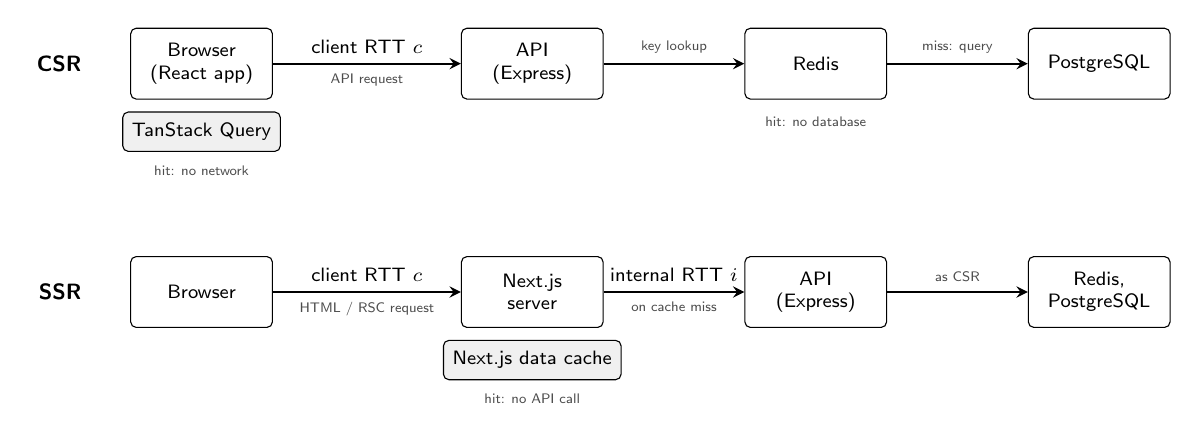
\begin{tikzpicture}[
  font=\sffamily\scriptsize, >=stealth,
  box/.style={draw, rounded corners=2pt, minimum height=9mm, minimum width=18mm, align=center, fill=white},
  cache/.style={draw, rounded corners=2pt, minimum height=5mm, align=center, fill=black!6},
  lane/.style={font=\sffamily\footnotesize\bfseries, anchor=east},
  hop/.style={->, thick},
  note/.style={font=\sffamily\tiny, text=black!70, align=center}]

% ---------------- CSR lane ----------------
\node[lane] at (0,0) {CSR};
\node[box] (cb) at (1.4,0) {Browser\\(React app)};
\node[cache, below=1.5mm of cb] (tq) {TanStack Query};
\node[note, below=0.5mm of tq] {hit: no network};
\node[box] (ca) at (5.6,0) {API\\(Express)};
\node[box] (cr) at (9.2,0) {Redis};
\node[note, below=1mm of cr] {hit: no database};
\node[box] (cd) at (12.8,0) {PostgreSQL};
\draw[hop] (cb) -- node[above]{client RTT $c$} node[below,note]{API request} (ca);
\draw[hop] (ca) -- node[above,note]{key lookup} (cr);
\draw[hop] (cr) -- node[above,note]{miss: query} (cd);

% ---------------- SSR lane ----------------
\node[lane] at (0,-2.9) {SSR};
\node[box] (sb) at (1.4,-2.9) {Browser};
\node[box] (sn) at (5.6,-2.9) {Next.js\\server};
\node[cache, below=1.5mm of sn] (nd) {Next.js data cache};
\node[note, below=0.5mm of nd] {hit: no API call};
\node[box] (sa) at (9.2,-2.9) {API\\(Express)};
\node[box] (sr) at (12.8,-2.9) {Redis,\\PostgreSQL};
\draw[hop] (sb) -- node[above]{client RTT $c$} node[below,note]{HTML / RSC request} (sn);
\draw[hop] (sn) -- node[above]{internal RTT $i$} node[below,note]{on cache miss} (sa);
\draw[hop] (sa) -- node[above,note]{as CSR} (sr);
\end{tikzpicture}
}
\caption{Request paths of the two rendering modes through the cache layers. Each cache outcome ends the path at a different point; the model's network term counts the client round trip $c$ and internal round trip $i$ on the remaining path. \emph{Initial load}: CSR fetches the document, then the JavaScript bundle (up to six connections per origin; one under HTTP/2), then calls the API on a new connection; SSR fetches the document on a new connection, and the server fetches the data before responding. \emph{Navigation}: CSR changes the URL and makes one API request on a warm connection, or none on a browser-cache hit; SSR makes one RSC request on a warm connection. Data-visible time ends at the first frame after the first data row enters the DOM.}
\label{fig:arch}
\Description{Two rows of boxes. The CSR row: browser with a TanStack Query cache, an arrow labelled client RTT to the API, then Redis, then PostgreSQL. The SSR row: browser, an arrow labelled client RTT to the Next.js server with its data cache, an arrow labelled internal RTT to the API, then Redis and PostgreSQL. Notes mark where each cache hit ends the path.}
\end{figure}

\paragraph{Testbed and networks.}
All services run in Docker containers; each link (client--web, client--API, web--API) is a separate network whose delay and rate are set with \texttt{tc netem}. A Playwright~1.56 Chromium client drives sessions. Real-network tests route the client's traffic through a remote host acting as a layer-3 relay (round trips of about 250--530\,ms); one further real path runs from a home broadband connection. Concurrency and CPU-throttling tests pin each service to a dedicated core of a Linux x86 host.

\paragraph{Measurement.}
A \texttt{MutationObserver} registered before any body content records the insertion of the first data row, and a \texttt{requestAnimationFrame} plus \texttt{MessageChannel} callback the next frame. At the insertion instant the page also records every displayed row's identifier and value and the identifier of the API response that produced them.

\paragraph{Serving layer per view.}
Each view is classified by the layer that served it, from identifiers carried out of band: a CSR view without a browser-cache request is a browser hit, otherwise the API log of that request shows a Redis hit or a database read; an SSR view whose displayed response was produced by the API before the view started came from the framework cache, otherwise the API log of that response shows a Redis hit or a database read. (A replay test on the server side alone misclassifies stale-while-revalidate: Section~\ref{sec:pitfalls}.)

\paragraph{Writes and the staleness oracle.}
A seeded writer updates records (catalogue: stock of a product on the workload's pages; every write increments a value) and logs each commit. Push invalidation deletes the Redis key and revalidates the page's framework-cache tag on each write; TTL invalidation relies on expiry. A view is stale if any displayed value differs from the database value at the display instant, reconstructed from a snapshot taken before the writer starts and the write log. Every one of the \AfiveViews{} views of the accepted staleness tests captured its full table; no displayed value was ever ahead of the database, also with the write log shifted by $\pm$20\,ms, which changes the stale share by at most \AfiveShiftMax{}.

% =====================================================================
\section{Pilot observations}
\label{sec:pilot}

A pilot (96 runs, 6{,}912 actions; 2 modes $\times$ 4 cache combinations $\times$ 2 RTTs $\times$ 2 workloads $\times$ 3 seeds) motivated the model.
Behind the Next.js data cache, Redis's conditional hit ratio was 0.00: a shared upstream cache absorbs every repeated key, the filtering effect of cache-hierarchy theory~\cite{che2002hierarchical,fofack2014ttl}, here in a default configuration; a per-user browser cache leaves Redis almost all of its value.
Initial load depends on the rendering path (SSR showed data 153\,ms sooner at RTT~0 and 1{,}093\,ms sooner at 170\,ms), while caches changed it by under 1\%.
Navigation has a crossover: with browser caching, CSR navigation beats SSR roughly when the browser hit rate times the client round trip exceeds the server work the shared cache saves.

% =====================================================================
\section{Latency model}
\label{sec:model}

\paragraph{Structure.}
For action $a$ in mode $m$ served by layer $o$, with client round trip $c$ and internal round trip $i$:
\begin{equation}
\hat T(m,a,o;c,i) = T_0(m,a,o) + N(m,a,o;c,i) - N(m,a,o;0,0) + \rho_{m,a,o}(c),
\label{eq:model}
\end{equation}
where $T_0$ is the mean latency measured at RTT~0 for that path (CPU, rendering and server time), $N$ is the critical-path network time, and $\rho$ is an empirical residual interpolated over the client RTTs of an emulated calibration grid. An action whose serving layer is uncertain is predicted as $\sum_o P(o)\,\hat T(m,a,o)$ (Section~\ref{sec:outcomes}).

\paragraph{Critical paths.}
CSR initial: document (new connection) $\rightarrow$ JavaScript bundle $\rightarrow$ API request (new connection to the API origin). CSR navigation: one API request on a warm connection, or nothing on a browser hit. SSR initial: document (new connection), plus an internal API request on a framework-cache miss. SSR navigation: one RSC request on a warm connection, plus an internal request on a miss.

\paragraph{Transfers.}
A request on a new connection pays a handshake (one RTT for TCP; two with TLS~1.3~\cite{rfc8446}). A response of $b$ bytes takes TCP slow-start rounds from an initial window of ten segments~\cite{rfc6928} (1{,}448-byte MSS), plus serialization $8b/\text{bw}$.

\paragraph{The JavaScript bundle and the connection race.}
Chromium loads the bundle's chunks over up to six connections per origin; the largest chunk runs either on the reused document connection (whose window has grown) or on a new connection (one more slow-start round), and which becomes free first depends on path micro-timing. The bundle term is $E[\text{bundle}](c) = p\,B_{\text{new}}(c) + (1-p)\,B_{\text{reused}}(c)$, with $B_{\text{new}}, B_{\text{reused}}$ observed per race group in calibration and $p$ measured on the target path before each run from eight probe loads of a page no workload uses. Under HTTP/2~\cite{rfc9113} all chunks share one connection and the bundle term is a single calibrated curve.

\paragraph{Inputs per run.}
Frozen calibration; the declared workload; client and internal RTT from TCP-connect probes before the run; the race probability $p$; and, where bandwidth is not fixed, the bottleneck bandwidth (two calibrated bandwidth levels, linear in $1/\text{bw}$ between them).

\paragraph{Concurrency.}
For $N$ concurrent users we extend the model with exact mean value analysis~\cite{reiser1980mva} over three single-core stations; queue lengths use each station's total CPU demand per action and each action's latency grows by its on-path demand times the queue length it meets, with load-dependent demand.

% =====================================================================
\section{Serving layer and staleness}
\label{sec:stale}
\label{sec:outcomes}

\paragraph{Timeline.}
The model replays the declared sessions on a timeline whose display gaps (time between consecutive views) are calibrated without writes, per mode, action and serving layer, as a linear function of the client RTT. Each cache entry carries its fill time and $\tau$, the instant at which its data was guaranteed equal to the database. The layers follow their documented semantics: a database read gives $\tau$ = request time; a Redis TTL entry serves while younger than $T$; a push-invalidated entry is deleted on each write to its page; the framework cache with revalidation time $R$ serves its entry and refreshes it in the background once it is older than $R$ (stale-while-revalidate~\cite{rfc9111}); a browser-cache revisit shows the cached entry and refetches in the background once it is older than $S$. Two timings are approximations: a framework background refresh is taken to replace its entry when it is issued, although it lands only after the internal fetch (which matters only for another request to the same page within those tens of milliseconds), and a request is taken to reach the server half a round trip plus rendering before its data are displayed.

\paragraph{Serving layer.}
Browser and framework TTL hits are determined by the timeline. A push-invalidated entry exists when a view arrives unless a write reached its page since the entry's last access, so the view is served by the next layer down with probability $1-P_0(\Delta)$, where $\Delta$ is the time since the last access and $P_0$ the write process's no-write probability below. The model thus predicts, per view, a distribution over browser hit, framework hit, Redis hit and database read; with sequential users, cold caches and no expiry within a run, the distribution is degenerate and analytic (criterion C4 of Section~\ref{sec:protocol} checks it).

\paragraph{Latency with server work.}
A view's latency is the calibrated no-write latency of its serving layer plus $d\,P(\text{db})$, where $d$ is the added server work per database read; the display gap grows by the same amount.

\paragraph{Staleness semantics.}
\begin{proposition}
\label{prop:stale}
Let the displayed data of a view be equal to the database at instant $\tau$, displayed at instant $t>\tau$. Assume (i) every write changes exactly one record and increases its displayed value, so no value returns to an earlier state; (ii) a write reaches the records shown on the view's page with probability $q$, independently of everything else; (iii) the oracle compares at $t$. Then the view is stale if and only if at least one write reached its page in $(\tau,t]$, and
\[ P(\text{stale}) = 1 - P_0(t-\tau), \qquad P_0(w) = E\!\left[(1-q)^{N(w)}\right], \]
where $N(w)$ is the number of writes of the process in a window of length $w$. For a Poisson process of rate $\lambda$, $P_0(w)=e^{-\lambda q w}$.
\end{proposition}
\begin{proof}
If no write reaches the page in $(\tau,t]$, every displayed value equals the database at $\tau$ and, unchanged since, at $t$. If at least one does, the record it changed has a larger value at $t$ than at $\tau$ by (i), so the display differs. Conditional on $N(w)=n$, by (ii) none of the $n$ writes reaches the page with probability $(1-q)^n$; taking the expectation gives $P_0$. For Poisson, $E[s^{N(w)}]=e^{-\lambda w (1-s)}$ with $s=1-q$.
\end{proof}
The formula is the classical one~\cite{cho2000freshness}; Quaestor applies the same thinning to a query's result set~\cite{gessert2017quaestor}. It fails when its assumptions fail: a write that restores an earlier value (an unfavourite after a favourite) can make a page fresh again, so the oracle must compare snapshots rather than count writes; a write to a record that is cached but not displayed does not make the view stale, which (ii) handles only if $q$ counts displayed records; and a page assembled from several responses at different instants has several $\tau$. In our catalogue workload every write increments a stock value of a product on the workload's pages ($q = 1/8$ per page), and all displayed rows come from one response inserted in one DOM mutation, so the proposition applies exactly. In the Conduit workload every write is a favourite by a user who has not favourited that article before; no favourite is removed during a run (favourites are reset to a baseline between runs), so the count only grows and (i) holds with $q$ the article's write probability. Workloads with edits or removals would need the snapshot comparison instead. Even with every cache off, a view can be stale: the data are read at the request and shown about half a round trip plus rendering later; the model predicts this window.

\paragraph{Other write processes.}
For periodic writes every $1/\lambda$ seconds with a uniformly random phase, $N(w)\in\{k,k+1\}$ with $k=\lfloor \lambda w\rfloor$ and $P(N=k+1)=\lambda w-k$. For bursty writes we use a two-state Markov-modulated Poisson process (rate $\lambda_{\text{on}}$ during exponentially distributed ON periods, none during OFF periods), for which $P_0(w)=\pi\, e^{(Q-\Lambda)w}\mathbf{1}$ with generator $Q$, $\Lambda=\operatorname{diag}(q\lambda_{\text{on}},0)$ and stationary distribution $\pi$. For a recorded trace we estimate $P_0$ nonparametrically from a training window, as the average of $(1-q)^{N(s,s+w)}$ over start times $s$. These are marginal probabilities; consecutive windows of one session are correlated, which leaves expected stale shares exact but not their variance. We checked each formula against Monte Carlo simulation of its process (agreement within 0.01).

% =====================================================================
\section{Choosing a policy}
\label{sec:select}

Given candidate policies $\mathcal{X}$, predicted mean latency $\hat L(x)$ and stale share $\hat S(x)$, the selector returns
\[ x^\star = \arg\min_{x\in\mathcal{X}} \hat L(x) \quad \text{subject to } \hat S(x)\le\varepsilon, \]
and abstains if no candidate is predicted feasible. A choice is scored on held-out observed values: its \emph{regret} is $(L(x^\star)-L(x^{\text{opt}}))/L(x^{\text{opt}})$, where $x^{\text{opt}}$ minimizes observed latency among observed-feasible candidates, and a choice whose observed stale share exceeds $\varepsilon$ is a \emph{violation}, reported with its magnitude instead of regret. We compare it with a framework-default policy, no caching, the best fixed policy from an earlier experiment, and direct tuning: one pilot run per candidate at the target condition, choosing by pilot means. Tuning needs those runs at every new condition, with live users exposed to every candidate; the model needs one calibration without writes. We do not model monetary cost: CPU work is not money, and our added server work $d$ is a sleep, not CPU consumption.

% =====================================================================
\section{Methodology}
\label{sec:protocol}

\paragraph{Prospective design.}
Each model version is calibrated on emulated data, frozen (code and parameters hashed), and tested on conditions and seeds never used for fitting or diagnosis; the harness writes the prediction for each run before the run starts. A version that passes must pass an independent replication. Failed versions are diagnosed from their data, and the diagnosed data may calibrate the next version, which then faces fresh tests; Appendix~\ref{app:ledger} lists every version and every fresh test. For the experiments added in this revision, three protocols (blocks, seeds, criteria, analysis code) were frozen and committed before their runs: a development block may only check the pipeline, each component has at most three development versions, and the final test and its replication run once. An audit of the record, carried out by the author and therefore not independent, but repeatable from the artifact, checks the commit times against the first run of every block, the frozen manifests against their hashes, the uniqueness of seeds, and the re-scoring of every block from its raw logs. It found two lapses that affected no prediction: an amendment and a change to the calibration script on the second host were committed one and two minutes after the start of the blocks they concern, although both were in place before any of that host's test runs.

\paragraph{Latency criteria.}
C1: mean relative error over cells $\le 3\%$. C2: every cell within $\max(5\%, 10\,\text{ms})$. C3: every SSR$-$CSR difference has the correct sign and lies within $\max(10\,\text{ms}, 10\%)$. C4: analytic cache outcomes match 100\%. C5: every prediction written before its run started. A cell is a combination of mode, cache setting, action type and network condition; its observed value is the mean over runs.

\paragraph{Staleness and joint criteria.}
W1: pooled mean absolute error over policy cells $\le 0.03$. W2: every cell within 0.05. W3: cells whose predicted stale shares differ by at least 0.05 are ordered correctly. W4: oracle integrity (no displayed value ahead of the database; writes logged; purge lag p99 $\le 20$\,ms). W5: predictions written before runs. L1: mean latency error over (cell, action) $\le 3\%$; L2: every (cell, action) within $\max(5\%,10\,\text{ms})$.

\paragraph{Serving-layer criteria.}
Predicted serving-layer distributions are scored with the multiclass Brier score $\frac1n\sum_v\sum_o (p_{v,o}-\mathbf{1}[y_v=o])^2$. O1: in every decile of predicted $P(\text{db})$ holding at least 100 views, the mean prediction is within 0.05 of the observed frequency. O2: the Brier score is below that of calibration-frequency probabilities (class frequencies per policy, action and revisit flag in the calibration runs). O3: the Brier score exceeds the forecaster's own expected score $\frac1n\sum_v\sum_o p_{v,o}(1-p_{v,o})$ by at most 0.03. A fixed Brier bound would be unattainable: whether a push-invalidated entry survives is random, and a perfectly calibrated forecaster scores about 0.08 on our workloads.

\paragraph{Baselines with equal information.}
Every baseline is fitted only on the calibration data of the model it is compared with and receives the same inputs per action: mode, action, predicted serving layer, client and internal RTT, bandwidth and CPU level where the model uses them, and the race probability (as an expectation over the two race groups). We fit a ridge regression on serving-layer indicators and their interactions with the inputs (degree 1 or 2), a random forest and gradient-boosted trees, with hyperparameters chosen by leaving one calibration RTT out. Earlier cache-blind baselines (a latency--RTT line per mode and action) are kept for reference.

\paragraph{Statistics.}
The independent unit is the run (one seed of one cell); actions within a run share a session, a cold start and a time window. Intervals are 95\% percentile intervals of a block bootstrap that resamples seeds (applied to all cells of a test together, preserving the pairing of methods), 10{,}000 resamples. Tests with two seeds per cell have wide and unreliable intervals, which we state where they occur. The predictors predict means; tail percentiles are descriptive.

% =====================================================================
\section{Latency accuracy}
\label{sec:accuracy}

Table~\ref{tab:tests} lists every fresh prospective latency test; Fig.~\ref{fig:scatter} shows all of their cells.

\begin{table}[t]
\centering\small
\caption{Every fresh prospective latency test. Mean and max are relative errors over cells; ``fails'' lists failed criteria; ``passed'' is the test's own verdict and ``accepted'' the version's (test and replication both pass).}
\label{tab:tests}
\begin{tabularx}{\textwidth}{>{\raggedright\arraybackslash}p{4.3cm} X r r l l l}
\toprule
Experiment & Conditions & Mean \% & Max \% & Fails & Passed & Accepted \\
\midrule
Emulated (v5) & netem, client 90/210 ms × internal 20/75 ms & 1.10 & 3.78 & -- & yes & yes \\
Emulated (v5), replication & netem, client 150/320 × internal 35/100 ms & 0.77 & 3.64 & -- & yes &  \\
Real path (v7) & relay + 40 ms & 0.61 & 1.15 & -- & yes & yes \\
Real path (v7), replication & relay + 20 ms & 1.08 & 2.27 & -- & yes &  \\
Real path, bandwidth input (v8b) & relay + 10 ms, uncapped & 0.62 & 2.23 & -- & yes & yes \\
\quad replication & relay + 40 ms, 15 Mbit/s & 0.70 & 2.38 & -- & yes &  \\
Real path, HTTPS + HTTP/2 (v9) & relay + 35 ms & 0.26 & 0.44 & -- & yes & yes \\
\quad replication & relay + 15 ms & 0.23 & 0.61 & -- & yes &  \\
HTTP/2, certificate trusted (v9b) & netem 80/330 ms & 1.20 & 6.01 & C2 & no & no \\
\quad replication & netem 200/450 ms & 0.18 & 0.53 & -- & yes &  \\
SvelteKit & netem 90/300 ms & 0.69 & 2.78 & -- & yes & yes \\
\quad replication & netem 200/350 ms & 0.33 & 0.90 & -- & yes &  \\
Heavier page & netem 90/300 ms & 1.23 & 2.91 & -- & yes & yes \\
\quad replication & netem 200/350 ms & 0.61 & 2.27 & -- & yes &  \\
Slow device, 4× CPU & netem 80/200 ms & 2.28 & 7.05 & C2, C4 & no & no \\
\quad replication, 2× CPU & netem 60/180 ms & 2.08 & 7.22 & C2 & no &  \\
Concurrency (P3), N = 4 & netem 100 ms & 3.16 & 3.71 & C1 & no & no \\
\quad replication, N = 8 & netem 100 ms & 2.00 & 3.41 & -- & yes &  \\
Concurrency (P4), N = 3 & netem 100 ms & 2.26 & 6.35 & C2 & no & no \\
\quad replication, N = 7 & netem 100 ms & 4.74 & 9.37 & C1, C2 & no &  \\
Home broadband (H3) & real home path + 5 ms & 8.26 & 26.21 & C1, C2, C3 & no & no \\
\quad replication & real + 25 ms & 5.28 & 11.39 & C1, C2 & no &  \\
\bottomrule
\end{tabularx}

\end{table}

\begin{figure}[t]
\centering
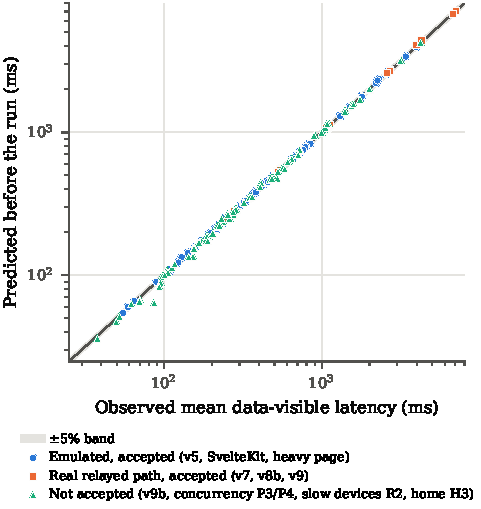
\includegraphics[width=0.48\textwidth]{figs/scatter.pdf}\hfill
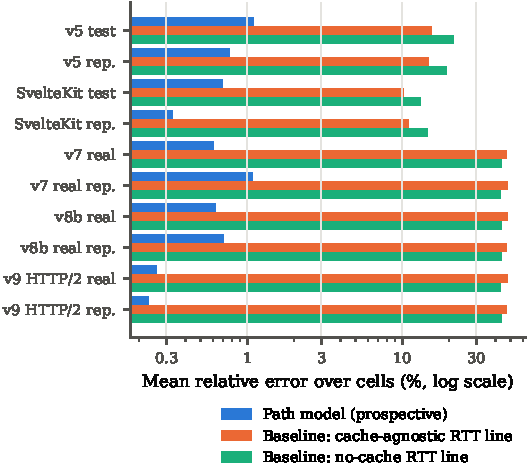
\includegraphics[width=0.48\textwidth]{figs/baselines.pdf}
\caption{Left: predicted (written before each run) vs observed mean data-visible latency for every cell of the latency tests in Table~\ref{tab:tests}, grouped by whether the model version was accepted. Right: mean error of the model and of baselines fitted on the same calibration data, per test.}
\label{fig:scatter}
\end{figure}

\paragraph{Emulated and real paths.}
The accepted emulated model predicts 9{,}216 actions per test at client RTTs of 90--320\,ms and internal RTTs of 20--100\,ms with 1.10\% (test) and 0.77\% (replication) mean error. A model recalibrated on the server host under emulation predicted a real relayed path within 2.3\%, but under-predicted CSR initial loads by 6--8\%: only the bundle phase differed, because a new connection won the race for the largest chunk in 75\% of real loads and 11\% of emulated ones (Section~\ref{sec:pitfalls}). With the race probability measured before each run, the model predicts the real path within 0.61\% and 1.08\%; with bandwidth probed per run, 0.62\% and 0.70\%; with HTTPS and HTTP/2 through a TLS-terminating edge, 0.26\% and 0.23\%. Recalibrated, the same equations predict a SvelteKit implementation (0.69\%, 0.33\%) and a heavier page (1.23\%, 0.61\%). These numbers hold for emulated paths and for a relayed path between data centres; on a consumer broadband path the errors are 5--8\% (Section~\ref{sec:limits}).

\paragraph{Where the accuracy comes from.}
We recomputed every prediction of these tests from the frozen inputs with terms removed (Fig.~\ref{fig:ablation}); the full variant reproduces the stored predictions exactly. Without the network and path terms (service time $T_0$ only) the error is \AoneServiceAll\%. Without the fitted residual $\rho$, the HTTP/1.1 tests' error rises from \AoneFullHone\% to \AoneNoRhoHone\%, so the residual is a small correction there. Replacing the measured race-split bundle curves with an analytic simulation of chunk dispatch raises real-path error to \AoneAbunReal\%: the connection race must be measured, not simulated. On the original HTTP/2 tests the residual carried \AoneNoRhoVnine\% of accuracy because it absorbed a test-harness certificate artifact (Section~\ref{sec:pitfalls}); with the artifact removed the structure alone reaches \AoneNoRhoVnineb\%. On the home path the residual hurt (\AoneFullHome\% with it, \AoneNoRhoHome\% without). Pooling $T_0$ over serving layers matters only where the server does real work: on the heavier page with 25\,ms of database work per read, error rises from \AoneNoRhoQ\% to \AonePooledQ\%.

\begin{figure}[t]
\centering
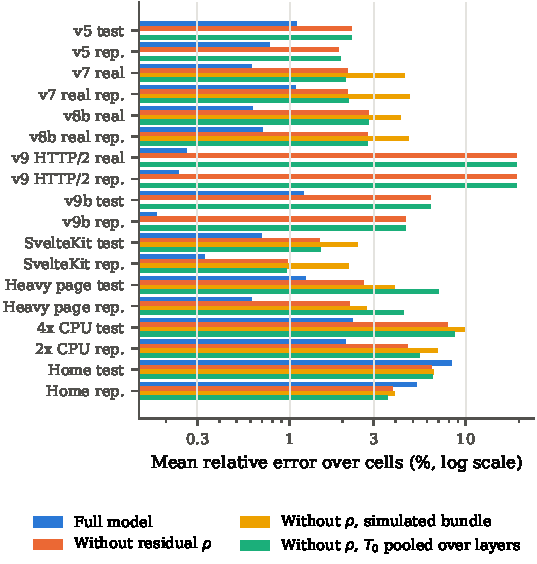
\includegraphics[width=0.48\textwidth]{figs/ablation.pdf}\hfill
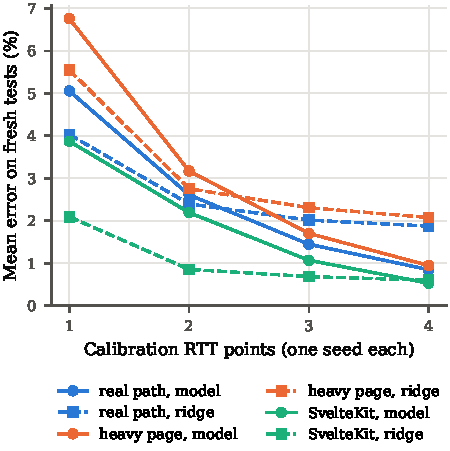
\includegraphics[width=0.48\textwidth]{figs/calibcost.pdf}
\caption{Left: mean error per test of the full model and with terms removed (retrospective, frozen inputs). Right: mean error on the fresh tests when the model and the equal-information ridge baseline are refitted on fewer calibration RTTs (one seed per point), against calibration runs.}
\label{fig:ablation}
\end{figure}

\paragraph{Equal-information baselines.}
Cache-blind baselines miss by 10--48\%. Once a baseline is told the serving layer, it is competitive: the ridge regression's mean error is \AtwoRidge\% across the \AtwoTests{} tests, and the model's is lower in \AtwoModelWins{} of them. Paired block-bootstrap intervals of the difference exclude zero in favour of the model in \AfourSig{} tests, include zero in \AfourTie{}, and favour the ridge baseline in \AfourRidgeSig{} (\AfourTwoSeed{} of the tests have only two seeds per cell, so their intervals are unreliable). The model's advantage is largest on real paths, where initial-load latency is not linear in RTT. Random forests and boosted trees, which cannot interpolate between sparse grid points, miss by \AtwoTrees\%. All test conditions lay inside the calibrated RTT range (\AtwoOutCells{} cells outside), so these data cannot show an extrapolation advantage. The conclusion is that conditioning on the serving layer accounts for most of the predictive power; the mechanistic terms add a smaller, real margin.

\paragraph{Calibration cost.}
Refitting on subsets of the calibration grid (Fig.~\ref{fig:ablation}, right) shows that one seed per grid point loses nothing, and that the structural model needs three or more RTT points: with three or four points (16--20 runs, under 25 minutes) it beats the ridge baseline on the real path and the heavier page; with one or two points the ridge baseline is better. On SvelteKit the ridge baseline is as good or better at every grid size.

\paragraph{Tails.}
The predictor targets means. On the real paths the 99th percentile of navigation latency is \AfourNavPninetyNine{} times the predicted mean, so the model should not be read as a tail predictor.

% =====================================================================
\section{Serving layers, staleness and policy choice}
\label{sec:fresh}

\paragraph{Earlier accepted tests.}
The staleness model was accepted with the latency model in four fresh tests (Table~\ref{tab:stale}), including a regime test in which each database read costs 25 or 100\,ms of server work. Run-level bootstrap intervals of the observed stale share contain the prediction in \AfourStaleIn{} of \AfourStaleCells{} cells. Scored retrospectively against the corrected serving-layer classification, the same frozen model predicted which layer served each view with Brier scores of \BoneOffBrier{} (skill \BoneOffSkill{} over calibration frequencies; the most likely layer was right for \BoneOffTop\% of views). On those tests a selector driven by the frozen predictions chose the observed-best feasible policy for every staleness limit (maximum regret \BfourOffMaxRegret\%), but so did two-run tuning: the nine candidate policies differed too much for the choice to be hard.

\begin{table}[t]
\centering\small
\caption{Earlier accepted staleness tests: pooled mean absolute error, worst cell, correct orderings and, for the regime experiment, latency error.}
\label{tab:stale}
\begin{tabular}{lrrrrr}
\toprule
Test & W1 MAE & W2 max & W3 & L1 & L2 max \\
\midrule
Writes, fast query: test (RTT 150, $\lambda$ 3/s) & 0.0113 & 0.0365 & 24/24 & -- & -- \\
\quad replication (RTT 60, $\lambda$ 1.5/s) & 0.0090 & 0.0217 & 22/22 & -- & -- \\
Regime: test (RTT 100, $d$ 25 ms) & 0.0130 & 0.0383 & 24/24 & 1.87\% & 4.91\% \\
\quad replication (RTT 200, $d$ 100 ms) & 0.0062 & 0.0180 & 27/27 & 0.95\% & 2.14\% \\
\bottomrule
\end{tabular}

\end{table}

\paragraph{New prospective tests.}
For this revision we froze a protocol and ran new blocks with seeds never used before (Table~\ref{tab:fresh}). In the catalogue blocks, 27 candidate policies (three without TTLs; six TTL-based policies at $\tau\in\{1,5,20,60\}$\,s, every TTL layer set to $\tau$) run under two access skews (Zipf $\alpha$ 0.6 and 1.0) with Poisson writes and 50 or 15\,ms of server work per database read; the test (client RTT 150\,ms) and the replication (80\,ms) use conditions the model never saw. The model is experiment X's frozen calibration with no refitting; it predicts for every view the serving-layer distribution, the latency and the staleness probability before the run.

\begin{table}[t]
\centering\small
\caption{Prospective tests added in this revision. W1: pooled staleness error; L1: mean latency error; Brier and skill: serving-layer prediction; regret: policy selection (mean over feasible decisions; for the near-threshold blocks, of the selector with a staleness margin; no selector with a margin violated a limit). ``Failed'' lists the pre-registered criteria the block missed. The near-threshold blocks predict from the session distribution only.}
\label{tab:fresh}
\begin{tabularx}{\textwidth}{>{\raggedright\arraybackslash}X r r r r r l}
\toprule
Block & W1 & L1 \% & Brier & Skill & Regret \% & Failed \\
\midrule
Catalogue, test (RTT 150, $d$ 50\,ms) & \revTWone & \revTLone & \revTBrier & \revTSkill & \revTRegret & \revTFails \\
\quad replication (RTT 80, $d$ 15\,ms) & \revRWone & \revRLone & \revRBrier & \revRSkill & \revRRegret & \revRFails \\
Write processes, test (periodic, on/off, trace) & \revBTwoTWone & \revBTwoTLone & \revBTwoTBrier & \revBTwoTSkill & -- & \revBTwoTFails \\
\quad replication & \revBTwoRWone & \revBTwoRLone & \revBTwoRBrier & \revBTwoRSkill & -- & \revBTwoRFails \\
Conduit, test (RTT 150) & \cdTWone & \cdTLone & \cdTBrier & \cdTSkill & \cdTRegret & \cdTFails \\
\quad replication (RTT 80) & \cdRWone & \cdRLone & \cdRBrier & \cdRSkill & \cdRRegret & \cdRFails \\
Conduit, second host, test (RTT 120) & \cdHTWone & \cdHTLone & \cdHTBrier & \cdHTSkill & \cdHTRegret & \cdHTFails \\
\quad replication (RTT 60) & \cdHRWone & \cdHRLone & \cdHRBrier & \cdHRSkill & \cdHRRegret & \cdHRFails \\
Near-threshold selection, model R2, test (RTT 120) & \revHTWone & \revHTLone & \revHTBrier & \revHTSkill & \revHTAwareRegret & \revHTFails \\
\quad replication (RTT 200) & \revHRWone & \revHRLone & \revHRBrier & \revHRSkill & \revHRAwareRegret & \revHRFails \\
\bottomrule
\end{tabularx}
\end{table}

\paragraph{Latency with predicted serving layers.}
With the serving layer predicted rather than known, latency remained accurate in every block: \revTLone\% and \revRLone\% mean error on the catalogue, \revBTwoTLone\% and \revBTwoRLone\% under other write processes, and \cdTLone\%, \cdRLone\%, \cdHTLone\% and \cdHRLone\% on Conduit (criteria L1 and L2 passed in all of them).

\paragraph{Serving layers.}
The predicted layer distributions had Brier scores of \revTBrier{} and \revRBrier{} on the catalogue (skill \revTSkill{} and \revRSkill{} over calibration frequencies; the most likely layer was right for \revTTop\% and \revRTop\% of views) and stayed within 0.03 of a calibrated forecaster's own expected score (O3) in every block. Calibration per probability decile (O1) failed in every block, by up to about 0.07. We diagnosed this after the fact on the catalogue blocks. First, the cache transitions follow the model's rule: for SSR with framework push invalidation, every view that followed a write to its page since the entry's last fill was fetched again (\diagPushTWriteFetched\%), and \diagPushTNoWriteCache\% of the others were served from the cache. Second, the write process is right: with the observed time since a page's last access, the Poisson no-write probability gives \diagPushTFormula{} and \diagPushRFormula{} database reads against \diagPushTObs{} and \diagPushRObs{} observed, while the model predicted \diagPushTPredR{} and \diagPushRPredR. About half of that excess came from the model counting an entry's exposure to writes until the view was displayed rather than until the request reached the server (correcting it gives \diagPushTPredRtwo{} and \diagPushRPredRtwo{}, so the correction removes about half of the excess; the rest (about 0.02) we have not explained, and candidate causes such as the server's render time before its cache read remain untested. We froze the corrected model (R2) and tested it on two fresh blocks with a new protocol: it passed O1, and every other staleness, latency and serving-layer criterion, in both (Table~\ref{tab:fresh}). Third, the criterion was close to the sampling noise: views of one run are correlated, and a bootstrap over runs puts the 95\% interval of a decile's deviation at $\pm$\diagNoiseTHalf{} on the catalogue test, so a perfectly calibrated forecaster would fail a 0.05 bound often; \diagNoiseTExcl{} of \diagNoiseTDeciles{} deciles (test) and \diagNoiseRExcl{} of \diagNoiseRDeciles{} (replication) had intervals excluding zero, with deviations up to \diagNoiseTMaxExcl. The serving-layer predictions are therefore calibrated to within about 0.05, with small real biases in a few deciles.

\paragraph{Staleness.}
Pooled staleness errors were \revTWone{} and \revRWone{} on the catalogue (W1 passed), but individual cells missed the 0.05 bound (\revTWtwo{} and \revRWtwo{} worst), and two of 1{,}134 orderings were wrong in the replication; the prediction lay inside the run-bootstrap 95\% interval of the observed stale share in \revTInside{} and \revRInside{} cells. Replacing the declared write rate by each run's realized rate changes the pooled error only from \diagDecrevTDeclared{} to \diagDecrevTRealized{} and from \diagDecrevRDeclared{} to \diagDecrevRRealized{}, so write-rate drift explains little of these misses; the largest ones are in long-TTL cells, where the stale share varies most from run to run. We separate known from estimated write processes. With the process given by its parameters, pooled errors were \revBTwoTPeriodicMae{} and \revBTwoRPeriodicMae{} for periodic writes and \revBTwoTOnoffMae{} and \revBTwoROnoffMae{} for on/off bursts. With the process estimated from the trace's past window, they were \revBTwoTTraceMae{} and \revBTwoRTraceMae{} (worst cell \revBTwoTTraceMax): the replayed test segments carried \diagTraceRate{} writes per second where the training window implied \diagTraceDeclared, and the rate error accounts for \diagDecTraceRate{} of the worst cell's \diagDecTraceTotal{} miss. A staleness prediction can be no better than its forecast of the write rate; where that forecast is uncertain, the selector below adds a margin rather than trusting the point estimate.

\paragraph{Workload knowledge.}
The predictions above used each run's declared sessions. Re-predicting the same blocks from the access distribution alone (Zipf $\alpha$ or the article popularity, the number of users and the session length; eight sampled session sets per run) left accuracy essentially unchanged: pooled staleness error \distrevTWoneDist{}, \distrevRWoneDist{}, \distcdTWoneDist{} and \distcdRWoneDist{} against \distrevTWoneDec{}, \distrevRWoneDec{}, \distcdTWoneDec{} and \distcdRWoneDec{} with the declared sessions, and run-mean latency error \distrevTLoneDist\%, \distrevRLoneDist\%, \distcdTLoneDist\% and \distcdRLoneDist\% against \distrevTLoneDec\%, \distrevRLoneDec\%, \distcdTLoneDec\% and \distcdRLoneDec\%. The model needs the distribution of sessions, not the sessions; the near-threshold test below uses distribution-only predictions throughout.

\paragraph{Choosing a policy.}
The selector met its criteria in every block that tested it. On the catalogue, its choices had mean regret \revTRegret\% and \revRRegret\% (worst \revTRegretWorst\%) over \revTDecisions{} feasible decisions per block, with no constraint violation; on Conduit, \cdTRegret\% and \cdRRegret\%, and on the second host \cdHTRegret\% and \cdHRRegret\%. For comparison on the catalogue test: tuning with one pilot run per candidate reached \revTTuningRegret\% (\revRTuningRegret\% on the replication) but needs 54 live runs at every new condition; the best fixed policy from the earlier experiment (SSR with framework and Redis push invalidation) \revTFixedRegret\% (\revRFixedRegret\%); no caching \revTNocacheRegret\% (\revRNocacheRegret\%); and the framework-default TTL policy violated the staleness limit in \revTDefaultViol{} of \revTDecisions{} decisions (on Conduit in \cdTDefaultViol{} of \cdTDecisions). On Conduit, whose article reads cost the server little, disabling caches cost only \cdTNocacheRegret--\cdHRNocacheRegret\%, so the decision there is mostly about freshness; on the catalogue, with 50 or 15\,ms of server work per read, it is about both. Selection succeeds although the stale shares it uses are only approximately right, because the candidates' latencies and stale shares are far apart compared with the prediction errors; near a crossover the margin would be smaller.

\paragraph{Decisions at the threshold.}
A selector whose candidates are far apart is easy to get right. To test it where predictions are least certain, a third protocol, frozen before its runs, used 16 candidates chosen to be close (TTLs of 2, 4 and 8\,s), a new access skew and server work, distribution-only predictions from model R2, and staleness limits placed at the predicted boundary: for every candidate on the predicted latency--staleness front, one limit 0.01 above and one 0.01 below its predicted stale share, both for all 16 candidates and for the TTL-only subset that an application without write hooks would face (8 decisions per block). The point selector chose the observed-best policy in \revHTNaiveRight{} and \revHRNaiveRight{} of 8 decisions, with mean regret \revHTNaiveRegret\% and \revHRNaiveRegret\%, but crossed the limit in \revHTNaiveViol{} and \revHRNaiveViol{} decisions (by at most 0.021; none was confirmed by the run-level interval). A selector that required the predicted stale share plus a margin of 0.05 (the 95th percentile of per-cell staleness error in the earlier blocks) to stay within the limit made no violation in any of the 16 decisions, at mean regret \revHTAwareRegret\% and \revHRAwareRegret\% (worst \revHRAwareWorst\%). The pre-registered bound of 5\% on that regret held in the test and was missed in the replication, so the near-threshold protocol as a whole was not accepted. Near a threshold, the predictions were accurate enough to keep a margin selector within its limits, and the margin cost about 4--6\% in latency. The margin is an empirical quantile of earlier errors, not a guarantee: it transfers to a new condition only if errors there resemble the earlier ones, and zero violations in \marginFiveDec{} decisions would bound the violation probability below about \marginUpper\% (one-sided 95\%) only if the decisions were independent trials with a common violation probability; they share a model, workloads and conditions, so this is an illustration of how little 16 decisions can establish, not a valid bound. The decisions were also insensitive to its exact value (a post-hoc check): margins of 0.02, 0.03 and 0.05 made the same \marginFiveDec{} choices (\marginTwoViol{} violations, mean regret \marginFiveRegret\%), no margin gave \marginZeroViol{} violations at \marginZeroRegret\% regret, and 0.07 abstained once at \marginSevenRegret\%.

\paragraph{A second, independently written application.}
On Conduit, whose backend, schema, queries and data shape we did not write (its front end is our instrumented Next.js application with the same cache layers, so this tests transfer across backends and workloads, not across front-end frameworks), the model recalibrated on Conduit (36 runs without writes) predicted latency within \cdTLone\% and \cdRLone\% on this machine and \cdHTLone\% and \cdHRLone\% on a second, Linux host, and its pooled staleness error was \cdTWone{}, \cdRWone{}, \cdHTWone{} and \cdHRWone. Without recalibration, the catalogue's calibration predicted Conduit's latency within \cdTZeroLone\% and \cdRZeroLone\% on the machine it was calibrated on, but missed by \cdHTZeroLone\% and \cdHRZeroLone\% on the second host, while staleness transferred in both places (pooled error \cdTZeroWone{}--\cdHRZeroWone): the serving-layer timeline and the write process carry over between applications and hosts, per-layer service times carry over between applications on one host but not between hosts. The second-host blocks each missed one criterion (\cdHTFails{} in the test, \cdHRFails{} in the replication), so cross-host transfer is not accepted under our criteria.

% =====================================================================
\section{Where prediction fails, and measurement pitfalls}
\label{sec:limits}

\paragraph{Consumer broadband.}
On a path from a home broadband connection, three model versions missed by 5--8\% mean error. Bandwidth varied 3--12\,Mbit/s between runs, request RTT drifted by up to 22\,ms within a run, and occasional slow requests raised mean navigation latency above any pre-run estimate while typical navigations matched (median 88\,ms observed vs 87\,ms predicted). We read this as path non-stationarity that pre-run probes cannot forecast; it is a hypothesis consistent with these diagnostics, not a demonstrated cause.

\paragraph{Concurrency.}
With $N$ users sharing one client core and single-core server stations, the queueing extension predicts fresh population sizes ($N=3,4,7,8$) within 2--5\% mean error (Fig.~\ref{fig:conc}); one version passed all criteria at $N=8$, but no version passed both its test and replication. Navigations are slightly under-predicted throughout; refitting moved errors between population sizes instead of reducing them.

\begin{figure}[t]
\centering
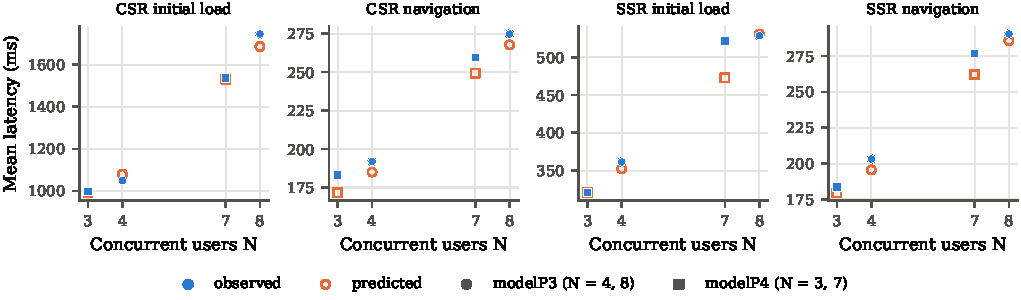
\includegraphics[width=\textwidth]{figs/concurrency.pdf}
\caption{Concurrency: observed and predicted mean latency per action type for fresh population sizes; two model versions (P3 at $N=4,8$; P4 at $N=3,7$).}
\label{fig:conc}
\end{figure}

\paragraph{Throttled devices.}
With Chromium CPU throttling calibrated at $1\times$ and $6\times$, fresh tests at $4\times$ and $2\times$ gave 2.28\% and 2.08\% mean error, all navigations within 2.3\%, but initial loads at 60--80\,ms RTT were over-predicted by 4--7\%; these RTTs fall between grid points (40 and 120\,ms) where initial-load time is not linear in RTT. The HTTP/2 variant with a trusted certificate missed in the same region.

\paragraph{Measurement pitfalls.}
\label{sec:pitfalls}
\emph{Emulation shifts the connection race.} Under \texttt{netem} a new connection won the race for the largest chunk in 11\% of loads, on the real path in 75\%; emulation-based studies of bundle loading should measure connection assignment. \emph{Certificate handling adds two round trips.} Accepting a self-signed certificate through Playwright's \texttt{ignoreHTTPSErrors} delays every new TLS connection by about two RTTs (417\,ms vs 0.8\,ms at RTT 207\,ms) and made CSR initial loads 29\% slower; trusting the certificate by key removes it. \emph{Stale-while-revalidate defeats replay-based hit detection.} A server-side test that calls a response a cache hit only if it was rendered before misclassifies a background-refreshed entry, which is new but served from cache, as a miss; at 100\,ms of server work such ``misses'' were exactly as fast as hits. Classifying by the displayed response's origin fixes it. \emph{CPU quotas and Apple Silicon distort service times.} CFS quotas throttle bursts (database p99 58\,ms vs 17\,ms); on an Apple Silicon host the same code ran about 4.5\,ms slower per read when lightly loaded, which invalidated a concurrency and a throttling experiment there.

% =====================================================================
\section{Threats to validity}
Two applications, one of them on an independently written backend but sharing our instrumented Next.js front end, and their variants (a second front-end framework, SvelteKit, was tested on the catalogue only); headless Chromium only; real paths through one relay host and one home connection; the trace-driven workloads combine public timing or popularity data with synthetic record choice, so they are trace-inspired rather than production workloads; models are recalibrated per framework, application and environment; the heavier-page tests ran with 25\,ms of added database work per read in calibration and test. Predictions are conditioned on a workload description (the session distribution and the write process); when the write rate drifts from its history, staleness predictions drift with it. Prediction intervals and cache eviction under memory pressure were not evaluated.

% =====================================================================
\section{Conclusion}
Data-visible latency and staleness of cached CSR and SSR applications can be predicted from the request path: which layer answers, the round-trip times, the bytes, the bandwidth, the server's work and the write process. Knowing which layer answers is most of the prediction, and that can itself be predicted from the declared workload and cache policies. The predictions were accurate enough to choose a rendering and caching policy under a staleness limit about as well as live tuning did in our tests with 27 candidates, on two applications and two hosts, after a one-time calibration and short network probes and without running the candidates; near the threshold, keeping within the limits cost more latency than our pre-registered bound allowed in one of two tests. At the decision boundary itself, a margin taken from past errors kept every choice within its staleness limit at a few percent of latency. The predictions first missed some per-cell and calibration criteria we set in advance; a corrected model passed them on fresh tests, but prediction still fails when the path, the load or the write rate does not behave like its history. Because every prediction was written before its run, each of these conclusions, including the negative ones, was checked on conditions the models had not seen.

\section*{Artifact availability}
The testbed, harness, frozen models and protocols, per-run predictions, raw logs and evaluation outputs, the analysis scripts and a script that re-scores every test from the raw logs are archived on Zenodo (\href{https://doi.org/10.5281/zenodo.23512120}{doi:10.5281/zenodo.23512120}, which resolves to the latest version; this paper uses version 1.1.1) and developed at \url{https://github.com/Istiak-A-Tashrif/cached-csr-ssr-latency}.

\begin{acks}
The author used a generative AI tool (Claude, Anthropic) to assist with implementing the testbed and analysis code, running and analyzing the experiments, producing the figures, and drafting and editing the text. The author directed the research and is responsible for all content.
\end{acks}

\bibliographystyle{ACM-Reference-Format}
\bibliography{refs}

\appendix
\section{Every model version and fresh test}
\label{app:ledger}
Table~\ref{tab:ledger} lists every model version, the reason it was created, the fresh tests it faced and the outcome. Diagnosed data from a failed test may calibrate the next version but never scores it.
{\footnotesize
\begin{longtable}{>{\raggedright\arraybackslash}p{1.25cm} >{\raggedright\arraybackslash}p{4.4cm} >{\raggedright\arraybackslash}p{3.2cm} >{\raggedright\arraybackslash}p{3.6cm}}
\caption{Model versions and their fresh tests (mean / max relative error, \%, and failed criteria).}\label{tab:ledger}\\
\toprule
Version & Change and motivation & Fresh tests (mean / max \%) & Outcome \\
\midrule
\endfirsthead
\toprule
Version & Change and motivation & Fresh tests (mean / max \%) & Outcome \\
\midrule
\endhead
\bottomrule
\endlastfoot
\multicolumn{4}{l}{\emph{Latency, emulated paths (macOS host)}}\\
v1 & Pilot path model & 1 test (max 39.4) & Superseded before criteria existed \\
v2 & Analytic cache outcomes; slow-start transfers & 1 test (3.3 / 11.8) & Superseded before criteria existed \\
v3 & TCP-connect RTT probes; warm-up page & stopped part-way & Stopped (author decision) \\
v4 & Connection-aware bundle dispatch; serialization & 3.68 / 11.88 (C1, C2) & Not accepted; criteria fixed before scoring \\
v5 & Residual $\rho$ over client RTT & 1.10 / 3.78; rep 0.77 / 3.64 & \textbf{Accepted} \\
\multicolumn{4}{l}{\emph{Latency, real relayed path (Linux host)}}\\
v6 & v5 recalibrated under emulation on the server host & 2.28 / 7.74 (C2, C3); rep 2.34 / 7.01 (C2) & Not accepted: connection race \\
v7 & Race probability measured before each run & 0.61 / 1.15; rep 1.08 / 2.27 & \textbf{Accepted} \\
v8 & Bandwidth as a measured input & 0.64 / 2.04; rep 0.88 / 2.51 (C3) & Not accepted: SSR navigation offset \\
v8b & v8 plus an SSR-navigation transfer offset from used real-path runs & 0.62 / 2.23; rep 0.70 / 2.38 & \textbf{Accepted} \\
v9 & HTTPS + HTTP/2 (TLS handshake, one connection) & 0.26 / 0.44; rep 0.23 / 0.61 & \textbf{Accepted} (residual absorbed a certificate artifact) \\
v9b & v9 with the certificate trusted & real path invalid (RTT 490--1{,}700\,ms); emulated 1.20 / 6.01 (C2); rep 0.18 / 0.53 & Not accepted (miss below the grid) \\
\multicolumn{4}{l}{\emph{Latency, transfer and limits}}\\
S & v7 equations recalibrated for SvelteKit & 0.69 / 2.78; rep 0.33 / 0.90 & \textbf{Accepted} \\
LQ & v7 equations for a heavier page & 1.23 / 2.91; rep 0.61 / 2.27 & \textbf{Accepted} \\
R & CPU throttling, two calibrated levels (macOS) & 3.26 / 5.05; rep 6.18 / 12.44 & Invalid: load-dependent core speed \\
LR2 & R repeated on pinned Linux cores & 2.28 / 7.05 (C2, C4); rep 2.08 / 7.22 (C2) & Not accepted; iteration stopped \\
C & Concurrency, MVA (macOS) & 10.79 / 13.61; rep 15.92 / 18.68 & Invalid: load-dependent core speed \\
P & MVA on pinned cores & 11.98 / 38.17; rep 26.56 / 83.78 & Not accepted: launch bursts, total demand \\
P2 & Launch barrier; on-path vs total demand & 2.70 / 8.84 (C2); rep 8.86 / 15.95 & Not accepted: load-dependent demand \\
P3 & Load-dependent demand & 3.16 / 3.71 (C1); rep 2.00 / 3.41 & Not accepted (replication passed) \\
P4 & P3 refitted on all barrier-era runs & 2.26 / 6.35 (C2); rep 4.74 / 9.37 & Not accepted; iteration stopped \\
H & Home broadband path & 6.76 / 7.90; rep 3.69 / 8.63 & Not accepted \\
H2 & Bandwidth levels; request-level RTT & 5.31 / 11.54; rep 6.36 / 22.58 & Not accepted: short probe read low \\
H3 & Pinned server cores; bundle-equivalent bandwidth & 8.26 / 26.21; rep 5.28 / 11.39 & Not accepted; iteration stopped \\
\multicolumn{4}{l}{\emph{Staleness (pooled absolute error)}}\\
W & Timeline staleness model & 0.063 (application bug); rep discarded unscored & Bug fixed; model unchanged \\
W (re-test) & Same frozen model, 8 seeds per cell & 0.011; rep 0.009 & \textbf{Accepted} \\
X & Joint latency and staleness with server work $d$ & 0.013, L1 1.87; rep 0.006, L1 0.95 & \textbf{Accepted} \\
\multicolumn{4}{l}{\emph{Revision: serving layer, staleness and selection (protocol frozen before the runs)}}\\
R & Experiment X's frozen calibration; declared write process; serving-layer distribution per view & catalogue \revTLone / \revRLone{} (latency); write processes \revBTwoTLone / \revBTwoRLone & Selection accepted; staleness and serving-layer gates not accepted (\revTFails; \revRFails; \revBTwoTFails; \revBTwoRFails) \\
RC & R with per-page write probability; recalibrated on Conduit (36 runs) & Conduit \cdTLone / \cdRLone; second host \cdHTLone / \cdHRLone & Selection accepted; other gates not accepted (\cdTFails; \cdRFails; \cdHTFails; \cdHRFails) \\
R2 & R with the push-exposure timing correction found post hoc on the catalogue blocks; predictions from the session distribution only & near-threshold \revHTLone / \revHRLone{} (latency) & All prediction criteria passed in both; margin selector 0 violations; regret bound missed in the replication \\
\end{longtable}

}

\end{document}
